\documentclass[10pt,journal,compsoc]{IEEEtran}
\usepackage[pdftex]{graphicx}
%\usepackage[sorting=none]{biblatex}
%\bibliography{references}
\usepackage{color}
\usepackage{dirtytalk}
%\usepackage{hyperref}

\hyphenation{op-tical net-works semi-conduc-tor}

\begin{document}
% thrhee
\title{Perceptual Evaluation of Dynamic Depth of Field \\ to Reduce Visual Discomfort in HMD}
% \title{Perceptual Evaluation of Visual Discomfort \\ using Dynamic Depth of Field in \\Head Mounted Displays}

\author{Kieran Carnegie and Taehyun Rhee
% thrhee: Kieran is the first author, Taehyun is the corresponding author
\IEEEcompsocitemizethanks{\IEEEcompsocthanksitem Taehyun Rhee is with the School of Engineering and Computer Science, Victoria University of Wellington, New Zealand \protect \\ E-mail: taehyun.rhee@ecs.vuw.ac.nz } }
%\IEEEcompsocitemizethanks{\IEEEcompsocthanksitem K. Carnegie is with the Department of Engineering and Computer Science, Victoria University of Wellington, New Zealand \protect \\ E-mail: kotarou@ecs.vuw.ac.nz } }

\IEEEtitleabstractindextext{%
\begin{abstract}
Head mounted displays (HMDs) are ideal devices for displaying immersive stereoscopic content, but they often cause significant visual discomfort, including eye fatigue, headaches, and nausea. A conflict between accommodation and vergence demands on stereoscopic displays is known to significantly contribute to this discomfort. We report the result of psychophysical experiments on the effectiveness of using dynamic depth of field (DoF) blur to reduce visual discomfort when using stereoscopic HMDs. Our DoF implementation adjusts the focal region in stereoscopic content based on the estimated view vector in real-time. Our implementation is realized in a commercial game engine. Participants reported a decrease of visual discomfort using a simulator sickness questionnaire (SSQ) when dynamic DoF blur is enabled. On average, we observe a reduction of the total sickness measure by approximately 30\% when dynamic DoF blurring is enabled on HMDs. 


\end{abstract}

\begin{IEEEkeywords}
% thrhee
Visual discomfort, Perception, Depth of Field, Head Mounted Display
% Simulator Sickness, Head Mounted Display, Depth of Field, Stereoscopic Display, Viewing Comfort
\end{IEEEkeywords}}

\maketitle
\IEEEdisplaynontitleabstractindextext
\IEEEpeerreviewmaketitle

\section{Introduction}

%%%%%%%%%%%%%%%%%%%%%%%%%%%%%%%%%%%%%%%%%%%%%%%%%%%%%%%%%%%%%%%%%%%%%%%%%% Problem definition
% Motivation of research domain
Recent advances in hardware technology have led to the production of consumer appropriate head mounted displays (HMDs) such as the Oculus Rift (the Oculus), ideal for personal use in immersive Virtual Reality (VR) applications including gaming, simulation, and film. Support from established companies such as Valve Software~\cite{valveVR} and the availability of the Oculus source development kit has resulted in a heretofore unseen, rapidly expanding ecosystem of applications, games and movies specifically designed for VR. This, coupled with the high quality and low price of the Oculus represents the first time VR has been so widely accessible in the market. \\

% What is the main issues of the research domain ?
Although HMDs represent an ideal set-up for immersive viewing of 3D stereoscopic content, they have a significant downside; people commonly report adverse physical reactions when using HMDs. These reactions include discomfort symptoms such as headaches, nausea, dizziness and eye-strain~\cite{howard02}, comparable to the symptoms commonly reported by sufferers of motion sickness. Collectively, these symptoms represent a condition referred to as \textbf{\textit{simulator sickness}}~\cite{mccauley84}. We refer to \textbf{\textit{visual discomfort}} as the specific subset of simulator sickness symptoms caused by visual stimuli. It has been found that up to 80\% of people experience these adverse reactions when using HMDs~\cite{Stanney03}.\\

% Why are they important and what is challenges ?
The human visual system uses a number of cues to infer depth and distance. Foremost among these cues are accommodation, the flexion of the lens in the eye required to form a focused image on the retina, and vergence, the inward rotation of the eyes required to form a single, binocular image. In stereo displays, these cues do not match, as the accommodation required to bring the physical HMD screen into focus will rarely match the vergence required to fuse the stereo image pair into a single binocular image, as shown in Fig.~\ref{fig:av-conflict}. This is caused by the requirement that the eyes converge to a variety of different depths, depending on the virtual depth of the observed object in the stereoscopic scene~\cite{rushton99}. The result of this mismatch is a conflict in the expected depths of visual stimuli, which is known to be a cause of visual discomfort~\cite{shibata11}. In stereoscopic 3D viewing, if the accommodative demand is fixed (as is the case for HMDs such as the Oculus) and a change in vergence demand occurs, a greater rate of change in the vergence demand will result in greater visual discomfort~\cite{kim14}. This indicates that it is not just the existence of conflict between accommodation and vergence demands that leads to discomfort: the requirement for the visual system to consistently re-adapt to new, conflicting demands is also a factor.\\ 

\begin{figure}
        \centering
            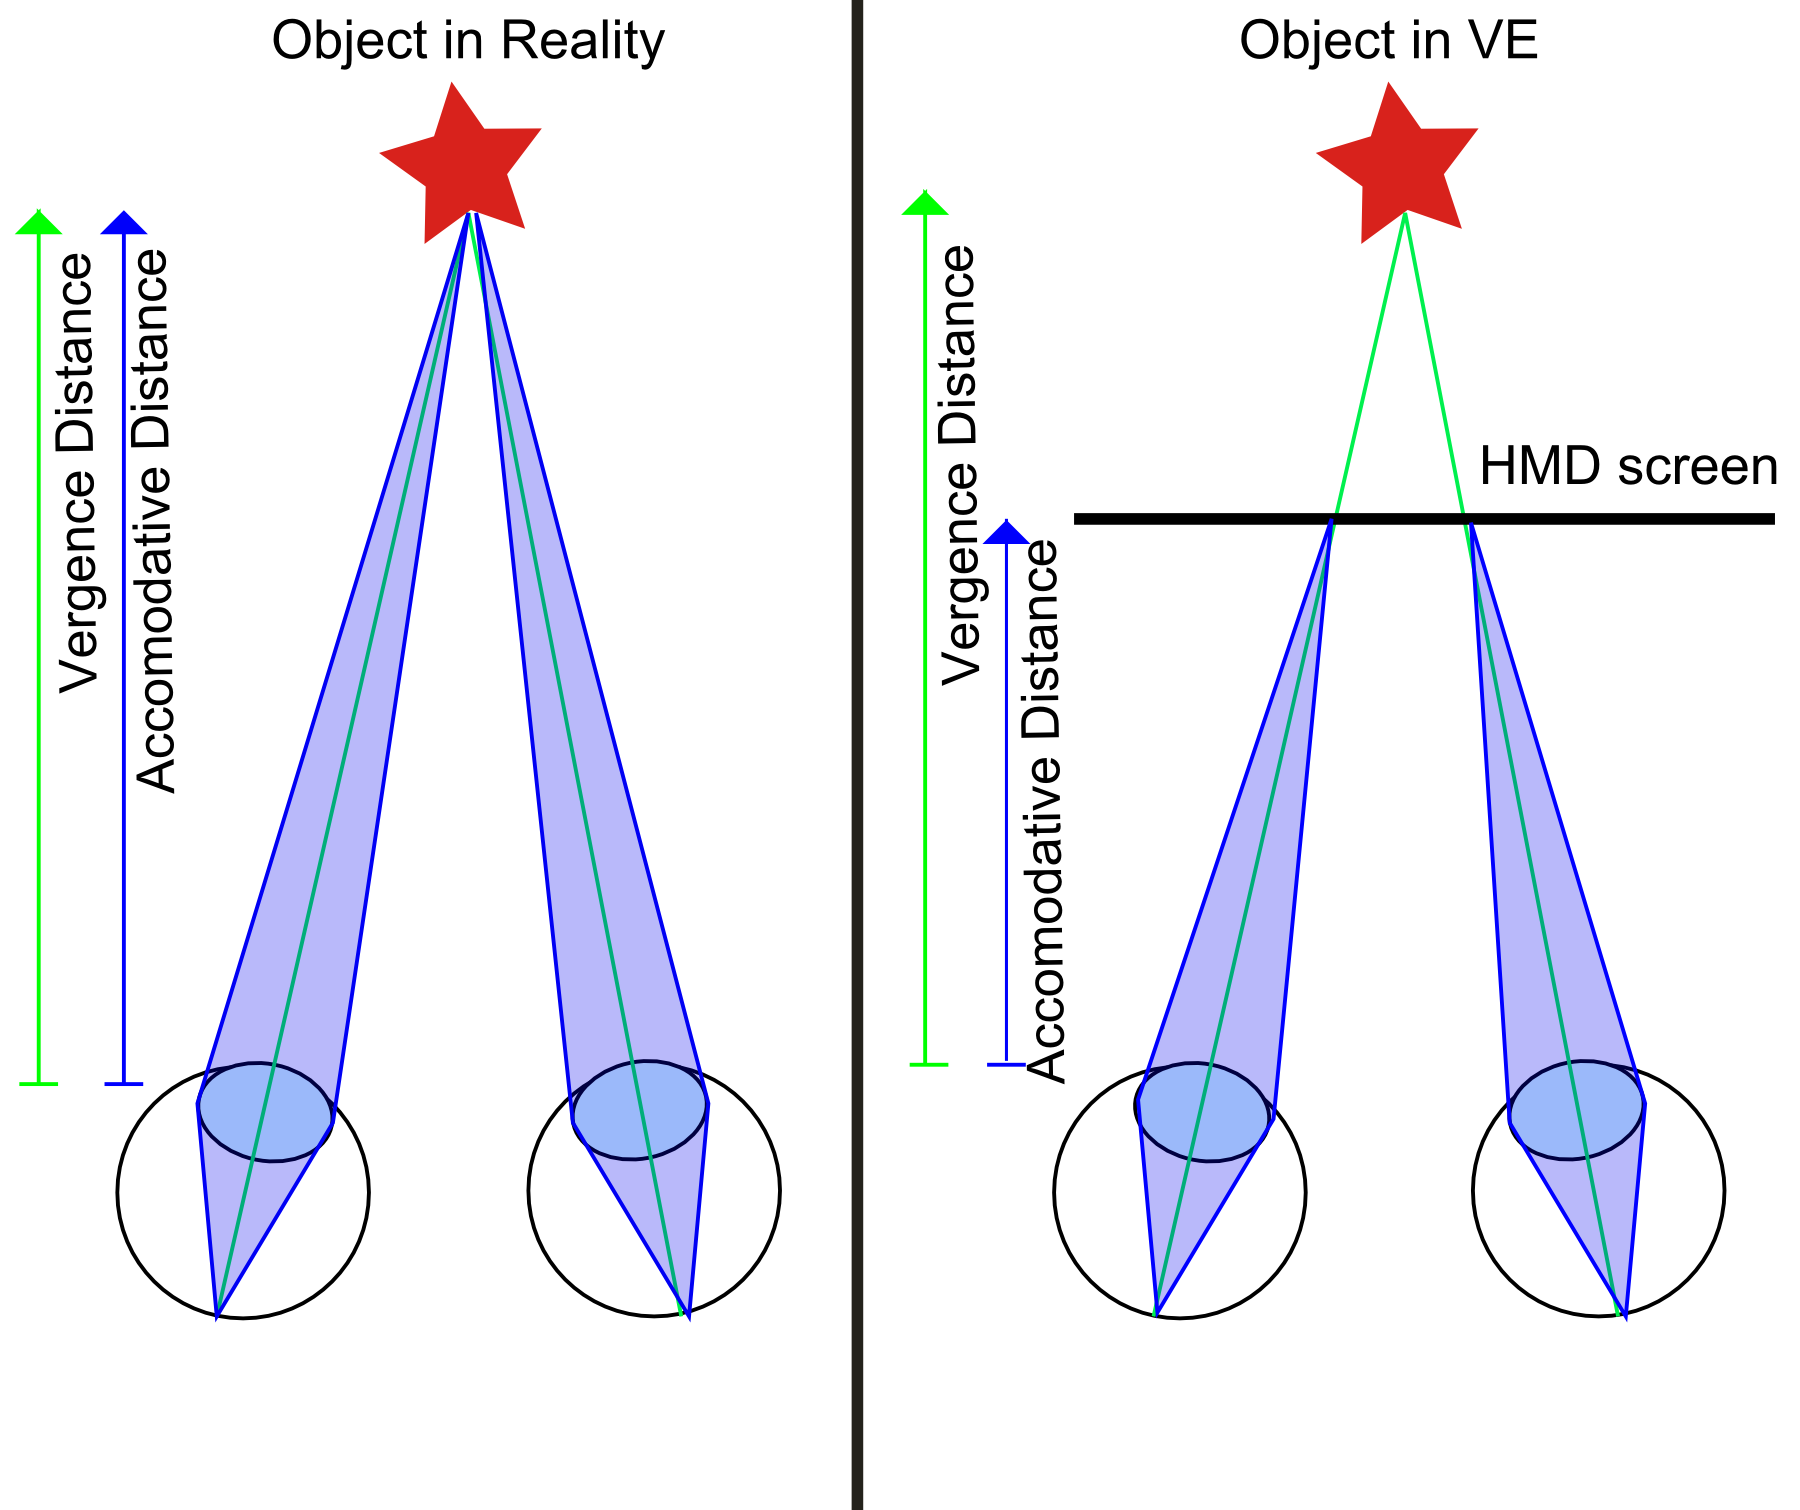
\includegraphics[width=0.45\textwidth]{images/vaconflict.png}
            \caption{An illustration of the accommodation-vergence conflict: comparing visual situations in real life (left) and when seeing objects in virtual environment (VE) on a HMD (right)}
            \label{fig:av-conflict}
\end{figure}

% Why is it challenging or What is the limitation of the previous work ?
%Moss and Muth\cite{moss08} report that modification to HMD hardware designed is required to reduces Visual Discomfort, a suggestion implementations such as Lanman and Luebke's\cite{Lanman13} light field display HMD follow. 
Following the suggestion that modifications to HMD hardware are required to reduce visual discomfort~\cite{moss08}, new hardware solutions such as the light field display HMD~\cite{lanman13} have been proposed. These implementations show promising results in reducing discomfort, but still have practical limitations including low display resolutions and pixel pitches. Gaze-contingent DoF can reduce visual discomfort when viewing stereoscopic content on LCD monitors viewed through a haploscope, according to a recent perceptual study~\cite{duchowski14}. This study used an external eye-tracking system to provide accurate calculation of participants gazes when using the haploscope. The requirement for such external hardware is intrusive in psychophysical evaluations of consumer level devices and may not accurately represent viewing conditions for users outside the lab. \\


In this paper, we perceptually evaluate the human visual system to show the effectiveness of dynamic DoF blur in mitigating visual discomfort when using stereoscopic HMDs. As far as we know, this is the first experimental report to investigate the effectiveness of dynamic DoF blur on HMDs. Our test system can be realised without any hardware modification and requires no usage of intrusive external devices: it relies only on positional data already captured by the Oculus. We implement a real-time dynamic DoF system in the Unreal Engine (Version 4)~\cite{unreal} and perform a series of psychophysical tests to show the effectiveness of the dynamic DoF blur on the Oculus. We use participant responses to questions about their subjective levels of discomfort as a metric, using a questionnaire based off the \say{Simulator Sickness Questionnaire (SSQ)}~\cite{kennedy93}. \\

\begin{figure*}
        \centering
            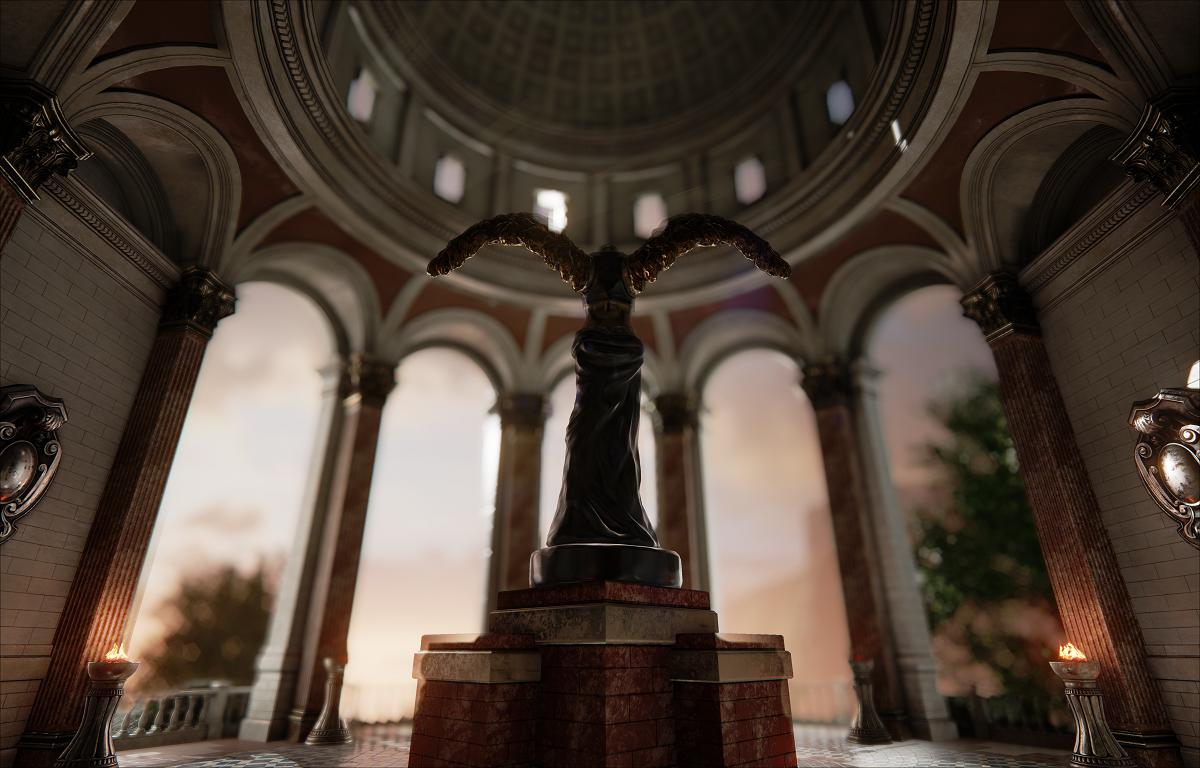
\includegraphics[width=0.45\textwidth]{images/lighton.png}
            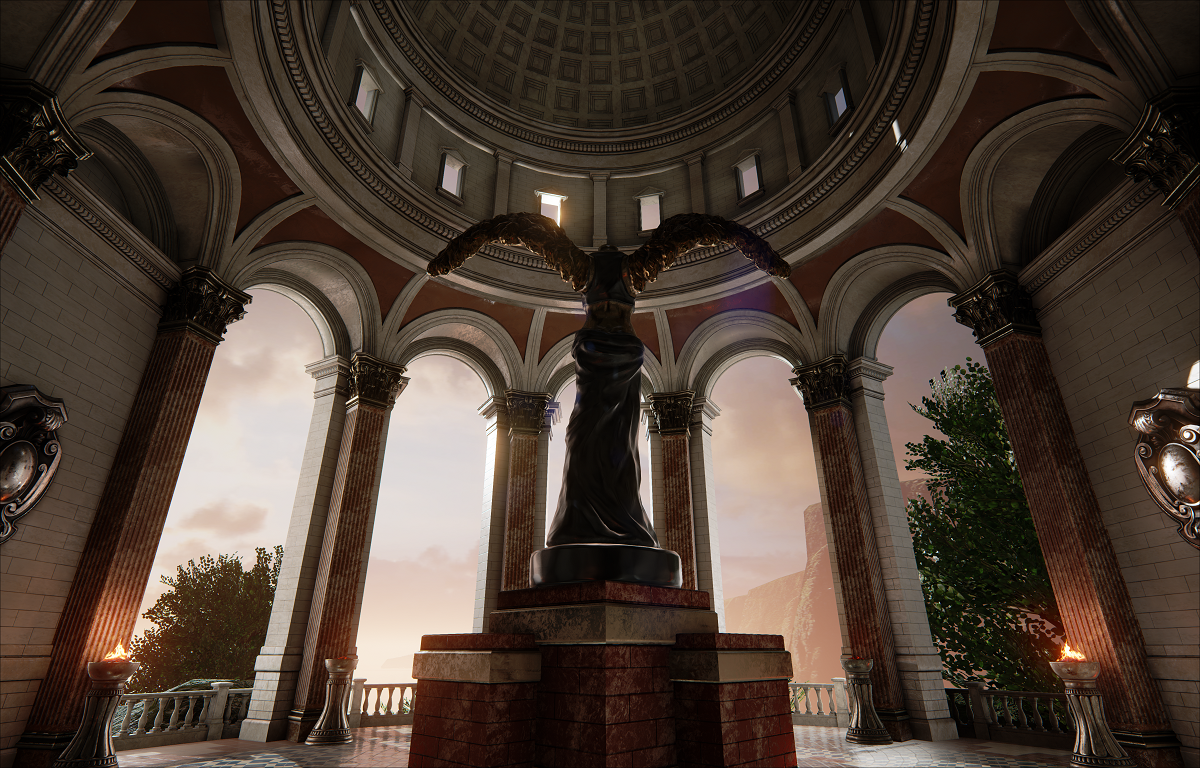
\includegraphics[width=0.45\textwidth]{images/lightoff.png}

            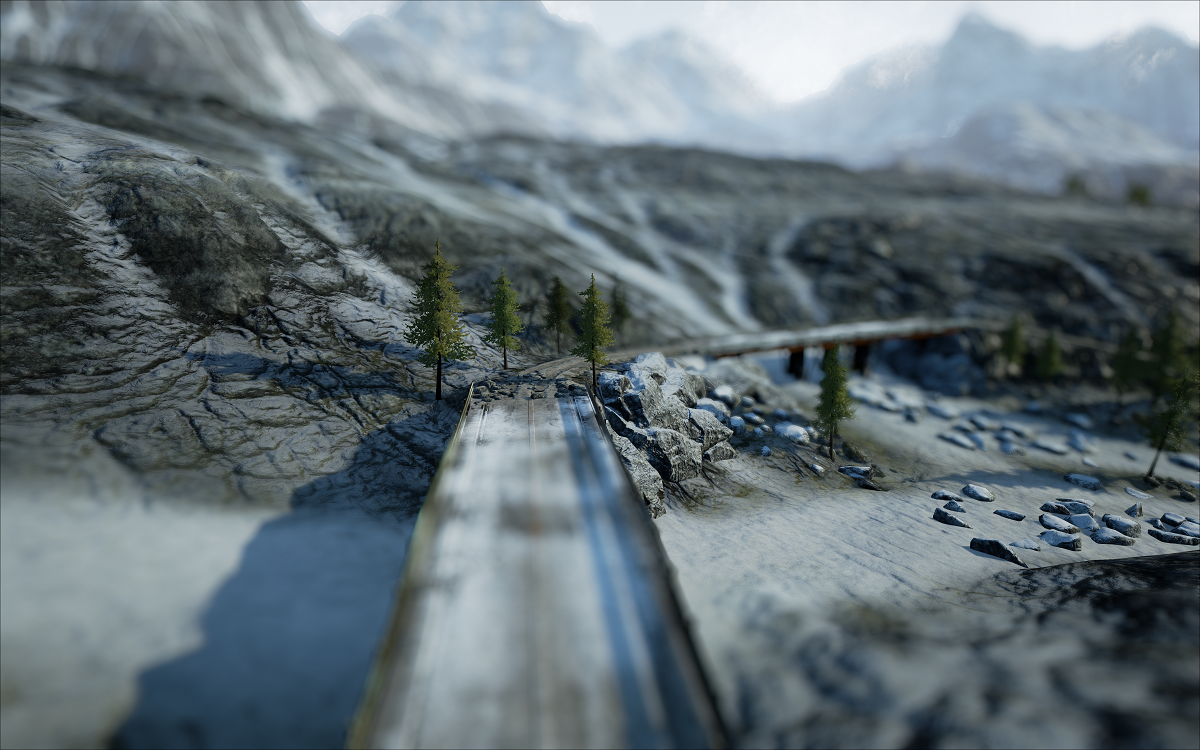
\includegraphics[width=0.45\textwidth]{images/landscapeOn.png}
            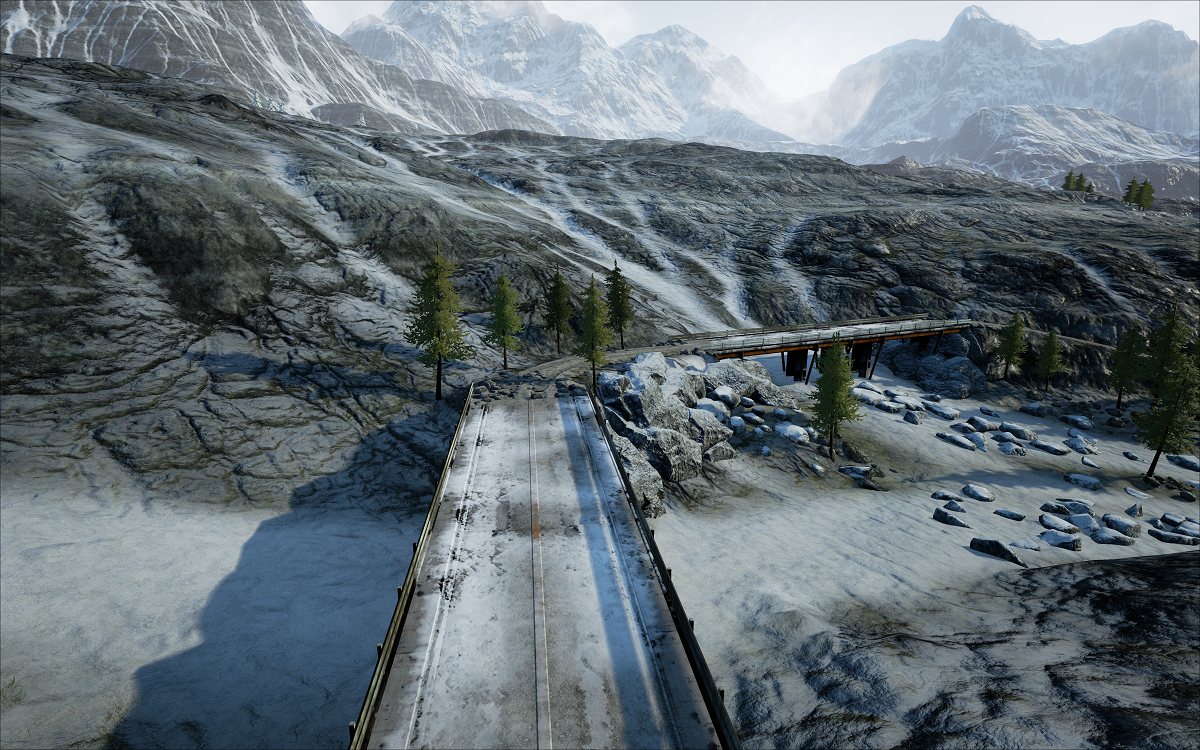
\includegraphics[width=0.45\textwidth]{images/landscapeOff.png}
            
            \caption{Sample screenshot of the test scenes (top Temple, bottom Mountainous), with DoF enabled (left) and disabled (right).}
            \label{fig:temple1}
\end{figure*}


%%%%%%%%%%%%%%%%%%%%%%%%%%%%%%%%%%%%%%%%%%%%%%%%%%%%%%%%%%%%%%%%%%%%%%%%%% OLD
%Recent advances in hardware technology have led to consumer level HMDs such as Oculus Rift \cite{oculusDK1}, ideal for immersive visualistion of virtual reality (VR) as a personal device. Support from openly-accessible Source Development Kit (SDK) software for the Oculus\cite{oculusSDK} has resulted in a growing ecosystem of games, movies, and VR applications. This, coupled with that high quality of the Oculus represents the first time VR has been so widely accessible in consumer market. \\

%Although HMDs are an ideal device to provide immersive stereovision in a wide range of field of view, the primary downside of HMDs is that people often report unpleasant reactions. These reactions, including symptoms such as headaches, nausea, dizziness and eyestrain\cite{howard:depthPerception} are often similar to those experienced by people who suffer from motion sickness, and are collectively termed \textbf{\textit{simulator sickness}} \cite{mccauley}. \cite{virtual:expect} indicates that as many as 80\% of people experience adverse effects when using HMDs. \\

%The human visual system uses a number of cues to infer depth and distance. Foremost among these cues are accommodation, the flexion of the lens in the eye required to form a focused image, and vergence, the rotation of the eyes to form a single, binocular image. In stereo displays, these two cues do not match: the eye accommodates to the physical screen in the screen, while the eyes converge towards a variety of depths, depending on the virtual depth of the observed object in the stereo scopic scene \cite{rushton99}. This leads to a conflict in the user's ocular system, which is known to be a cause of visual discomfort \cite{shibata:zone}. \cite{kim14} shows that in stereo 3D viewing, when the accommodative demand is fixed (as is the case for a HDM) and the vergence demand changes, a greater rate of change of the vergence demand results in a higher visual discomfort, a major contributing factors to Simulator Sickness, and as such mitigating this conflict is the main challenges to reduce visual discomfort in stereo scopic displays including HMDs. \\

%\cite{moss08} reported that modification to HMD hardware design are required to reduce Simulator Sickness, and Lanman and Luebke \cite{Lanman13} adapted light field displays to their HMD prototype for mitigating the problem. Although it shows a promising result, it still has many practical limitations such as display resolution and pixel pitches. Recently, \cite{Duchowski:2014:RVD:2628257.2628259} showed their perceptual test results reporting that gaze-contingent DOF can reduce the visual discomfort when viewing in stereoscopic display using LCD monitors arranged in haploscope. They used an external eye-tracker to provide pixel-accurate eye-tracking in their experiment. Such extra setup is intrusive in psychophysical test of consumer level devices.\\

% What is our solutions and contribution
%In this paper, we perceptually evaluate human visual system to show effectiveness of dynamic DOF blur to mitigate the visual discomfort when viewing in stereoscopic HMDs. As we know, this is the first experimental report to evaluate effectiveness of dynamic DOF blur in HMDs. Our test system can be realized without any hardware modification or external intrusive devices, as it only relies on positional data already captured by the Oculus. We implemented dynamic DOF \cite{dx9:dof} in Unreal Engine 4\cite{unreal} and performed a series of psychophysical test to show the effectiveness of dynamic DOF blur in Oculus, using participant responses to questionnaire \cite{ssq} on discomfort symptoms as a metric. On average, we showed a reduction of visual discomfort occurs when using dynamic DOF blur on HMD. Since our experimental setup does not require extra device or hardware modification, the result can be simply adapted in many applicatios viewed in general stereoscopic HMDs.


%%%%%%%%%%%%%%%%%%%%%%%%%%%%%%%%%%%%%%%%%%%%%%%%%%%%%%%%%%%%%%%%%%%%%%%%%% OLDEST
% The recent advances in hardware technologies release of the Oculus Rift DK1 (hereafter referred to as the Oculus) Development Kit brings, Virtual Reality (VR) technology to market at a price point (<\$400) suitable for reasonable consumer access. Support from companies such as Valve, who have released patches to popular games such as Half Life 2 and Team Fortress 2 to enable VR viewing modes, along with the availability of the openly-accessible SDK for the Oculus has resulted in a growing ecosystem of games, movies and applications designed with VR capabilities. This, coupled with that high quality of the Oculus represents the first time VR has been so widely accessible: prior VR implementations such as the Nintendo VirtualBoy or Vuzix VFX-1 suffered from poor execution and an extremely limited range of usable applications. \\

% The majority of VR implementations rely on a 3D stereoscopic display (S3D), in which each of a user's eyes are shown slightly differing images to simulate natural vision. This allows the VR device to provide a more immersive experience than traditional 2D display methods. Devices in which this S3D display is mounted to the user's head, instead of being placed in a fixed location like a traditional LCD computer screen are referred to as binocular Head Mounted Displays (HMDs), and are known to have several advantages, foremost of which is the screen's proximity to the user in a HMD occluding external visual stimuli, allowing the user to focus exclusively on the content shown on the S3D screen. Other varieties of HMD exist, including those that present an identical image to each eye (biocular) and those that only present one image (monocular), however we only focus on binocular HMDs. \\

% The primary downside of HMDs is that people often report unpleasant reactions to HMD systems. These reactions, including symptoms such as headaches, nausea, dizziness and eyestrain\cite{howard:depthPerception} are often similar to those experienced by people who suffer from Motion Sickness, and are collectively termed Simulator Sickness\cite{mccauley}. \cite{virtual:expect} indicates that as many as 80\% of people experience adverse effects when using HMDs. \\

% Given the rising popularity of consumer level VR, it is thus imperative that simulator sickness is  mitigated for the majority of vision-normal consumers to allow the continued growth of the applications.  The ideal solution for the current existence of a VR ecosystem should:\\
% \begin{itemize}
%	\item Be device agnostic. 
%	\item Require no purchase or installation of external devices to modify behaviour of current-market technologies. 
%	\item Allow application in both passive (such as film) and active (such as gaming) VR tasks. \\
%\end{itemize} 

%The current existence of a VR ecosystem where many separate developers are publishing VR ready content, and multiple VR devices (of which the Oculus is currently the most well known) exist, solutions for reducing Simulator Sickness optimally should:\\
%\begin{itemize}
%	\item Be device agnostic. 
%	\item Require no purchase or installation of external devices to modify behaviour of current-market technologies. 
%	\item Allow application in both passive (such as film) and active (such as gaming) VR tasks. \\
%\end{itemize} 

%Since HMDs display content at a very small distance from the viewers eyes ($<10cm$), something something low margin, extremes of vision.

% If any, what was the problems or limitations of the previous solutions ?
% These restrictions mean that prior implementations for reducing Simulator Sickness are insufficient. For example, \cite{Duchowski:2014:RVD:2628257.2628259} use a external eye-tracker to provide pixel-accurate eye-tracking in their solution, and \cite{moss2008characteristics} conclude that modification to HMD design and user behaviours are required to reduce Simulator Sickness. Furthermore, implementations that require eye tracking have to exclude users who are unable to calibrate the tracker properly, through either minor visual aberrations or unusual visual activity. \\


%%%%%%%%%%%%%%%%%%%%%%%%%%%%%%%%%%%%%%%%%%%%%%%%%%%%%%%%%%%%%%%%%%%%%%%%%% Summary and Contribution
% What is the proposed solution ? (overview of the methods)
% Adding in rationale for the method chosen. Not sure if this is the correct location or ot.
% The human visual system uses a number of cues to infer depth and distance. Foremost among these cues are Accommodation, the flexion of the lens in the eye required to form a focused image, and Vergence, the rotation of the eyes to form a single, binocular image. On HMDs, these two cues do not match: the eye accommodates to the physical screen in the HMD, ~6cm from the eye, while the eyes converge towards a variety of depths, depending on the virtual depth of the observed object in the S3D scene.\\

% Add an image here detailing the two, and how they conflict on the HMD

% This leads to a conflict in the user's ocular system, which is known to be a cause of visual discomfort \cite{shibata:zone}, a major contributing factors to Simulator Sickness, and as such we propose a system aimed at mitigating this conflict. \cite{Duchowski:2014:RVD:2628257.2628259} shows that blurred images (ie, images on the retina that either have failed to accommodate, or were artificially blurred) in the human visual system do not carry the same stimuli to fuse into a single binocular image as focused images do . 




\section{Related Work}

%Survey of HMD (briefly)
%Surveys of HMDs include those done by Rolland and Cakmakci\cite{rolland05:1} and Rolland and Hua\cite{rolland05:2}. 
HMDs provide an immersive viewing environment appropriate for VR applications, and can be classified according to the configuration of the HMD's screen and optics. According to previous surveys~\cite{rolland05:1,rolland05:2}, HMDs fall into three categories: stereoscopic, where the illusion of depth is created by delivering images rendered from different angles to each eye; monoscopic, where  identical content is delivered to each eye; and bioptic where only a single display is present that is viewed by both eyes. The Oculus~\cite{OculusDK1} that we used for this paper is a stereoscopic HMD.\\

\noindent \textbf{Simulator sickness:}
In 1958, findings on the incidence of symptoms similar to motion sickness in users of the 2-F2-H Hover Trainer, a simulator for training helicopter pilots were released~\cite{miller58}. These symptoms would later come to be grouped under simulator sickness, ``a term used to describe the diverse signs or symptoms that have been experienced by flight crews during or after a training session in a flight simulator''~\cite{mccauley84} which is now used to describe ``discomfort [occurring] in a simulator of any kind''~\cite{johnson05}. Simulator sickness symptoms can be split into three groups~\cite{kennedy93}: oculomotor symptoms such as eye-strain, blurry vision, and headaches; disorientation symptoms such as dizziness and vertigo; and nausea symptoms such as changes in salivation and stomach awareness. Some symptoms may contribute towards overall discomfort in more than one group: blurry vision can be considered to contribute to both the oculomotor and disorientation discomfort categories, for example.\\

Prior studies suggested specific hardware components such as helicopter simulator motion bases, or low update frequency CRT displays were responsible for causing simulator sickness~\cite{miller58}. It has since been found that simulator sickness symptoms also occur in HMDs~\cite{howarth97}, indicating such symptoms arise in a far greater variety of immersive VR applications than was initially expected.\\

\noindent \textbf{Causes of simulator sickness on HMDs: }
Previous studies have investigated factors that specifically lead to simulator sickness (as we refer to it, visual discomfort) on HMDs~\cite{kolasinski95, pausch92}. It was concluded that discomfort is caused by users undergoing motions that are abnormal when compared to reality (e.g. vection \cite{hettinger90}) or through the virtual environment not behaving in a manner that accurately simulates the expected visual stimuli. Early simulator sickness findings~\cite{miller58} support this as it was found that the more experience a pilot had in actual flight, the more severe their experienced discomfort would be in the simulator.\\

% condensed: as they would better understand what motions should be occurring during flight, and be more perturbed by the differences between simulation and actual flight.\\

\noindent \textbf{Reducing visual discomfort: }
It has been found that viewing monoscopic content, or stereoscopic content with a very small angle of difference between the two images (micro-stereoscopic) caused less discomfort compared to viewing identical stereoscopic content~\cite{ehrlich96}: removing and/or minimising the vergence cues for depth and distance estimation reduces discomfort. It was also found that occlusion of peripheral vision on HMDs is a contributor to visual discomfort~\cite{moss11}: not being able to view content external to the HMD screen exacerbates the sensory conflict between the vestibular and ocular systems. Following this, it was proposed that future HMDs do not entirely cover the visual field in order to reduce visual discomfort.\\

Other attempts to explicitly solve the accommodation-vergence conflict in stereoscopic displays have also used hardware based approaches involving set-ups such as multi-focal displays~\cite{akeley04, love09}, alternative lens systems~\cite{liu10}, or multi-lens systems~\cite{rolland05:2, lanman13}. These architectures all provide close-to-correct accommodation cues for multiple depths but their complex construction prohibits easy application to consumer level devices such as the Oculus at this time.\\

%During our survey, we could not find studys into solving the accommodation-vergence conflict using purely software factors on stereoscopic HMDs.\\

\noindent \textbf{Visual perception of DoF blur: }
Blurring effects are known to serve as a cue for perception of object size~\cite{held10}, and in conjunction with cues such as binocular disparity (featured in all stereoscopic implementations) also serve to alter perception of quantitative depth~\cite{mather96}. Adding blur gradients to simulate DoF and peripheral blur improves quality and realism of game play in a single display~\cite{hillaire08} and DoF blur can reduce rivalry from monocular regions in stereoscopic images~\cite{hoffman10}, indicating that DoF blur should decrease visual discomfort without negatively impacting the quality of the virtual environment.  \\

\textbf{Perceptual study of DoF to reduce accommodation-vergence mismatch: }
Focal cues including artificial blur and accommodation directly contribute to the quality of a 3D experience through the reduction of visual fatigue~\cite{shiwa96}. Furthermore, correcting these cues is one of the most important factors for viewing comfort~\cite{kooi04}. Correct focusing when viewing content on a stereoscopic display reduces visual fatigue and discomfort by lessening the strain caused by the accommodation-vergence conflict~\cite{hoffman08}. %Recent perceptual studies~\cite{duchowski14} show that visual discomfort can be reduced in stereoscopic displays through the use of DoF blur techniques that simulate the accommodative effect. % this has already been written, in the introduction.
During our survey, we could not find prior perceptual studies to report the impact of using DoF blur to reduce accommodation-vergence conflict in the specific case of stereoscopic HMDs.\\


%%%%%%%%%%%%%%%%%%%%%%%%%%%%%%%%%%%%%%%%%%%%%%%%%%%%%%%%%%%%%%%%%%%%%%%%%% OLD
%HMDs provide immersive visualization ideal for VR.  The type of the HMDs are often classified according to the optic and screen configurations, and well surveyed in \cite{Rolland_thepast, rolland05}. The screen on HMDs can be either stereoscopic (create the illusion of depth by sending images rendered from different angles to each eye), monoscopic (send the same image to each eye) or biopic (both eyes view the same display). The Oculus that we used in this paper is a stereoscopic HMD\cite{OculusDK1}.\\

%\noindent \textbf{Simulator Sickness:}
% this needs to link to HMDs
%Simulator sickness is referred to as the incidence of sickness symptoms associated with motion sickness, arising in the specific case where the user is interfacing with a visual display \cite{johnson}. The first occurrence of simulator sickness was reported on the first helicopter fight simulator, back in 1956 \cite{miller}. \cite{virtual:expect} indicates that as many as 80\% of people experience these adverse effects when using HMDs. The symptoms associated with simulator sickness on HMDs are broadly classified into three groups \cite{kennedy93}: 1) oculomotor symptoms such as eyestrain, blurry vision and headaches; 2) disorientation symptoms such as dizziness and vertigo and nausea symptoms; 3) changes in salivation and stomach awareness \cite{howard:depthPerception}. Some symptoms may contribute towards overall discomfort in more than one group: For example, blurry vision can be considered to contribute to both oculomotor and disorientation discomfort. We refer to \textbf{\textit{"Visual Discomfort"}} as the specific case of simulator sickness on HMDs related to human visual system.\\

%\noindent \textbf{Reason of Visual Discomfort: }
%Previous studies in \cite{mil:lit, mil:simsick}  have investigated factors that lead to the visual discomfort in HMDs.  The discomfort tends to be caused by either  the user to undergo motions that are abnormal when compared to experiences in reality (e.g. vection \cite{vection}), or through the presented scene on the display not behaving in a manner that accurately simulates the expected human visual system. 

%Shibata et al. \cite{shibata:zone} showed that the conflict between vergence and accommodation depth cues in stereoscopic displays cause visual discomfort. It is known that in typical viewing conditions, the vergence and accommodation effects in the human eye are tightly coupled. As like HMDs when the accommodative demand is fixed, a greater rate of change of the vergence demand results in a higher visual discomfort \cite{v:a}.\\

%\noindent \textbf{Reducing the visual discomfort: }

%\cite{stereovsmono} found that the viewing of monoscopic or micro-stereoscopic content on a HMD was less sickening, compared to viewing the same, stereoscopic content. This indicates that the removal of the accommodation-vergence conflict does increase viewer comfort. \cite{hmd:sick} concludes that the occlusion of peripheral vision on HMDs is a contributor of the visual discomfort, given that this occlusion prevents the viewing of sources external to the display in the HMD, furthering the sensory conflict between the vestibular and ocular systems, and thus recommend changing of the structure of HMDs to not entirely cover the visual field. The previous attempt to solve the accommodation-vergence mismatch do so through hardware based approaches. These hardware solutions tend to involve either multi-focal displays \cite{Akeley:2004:SDP:1015706.1015804, Love:09}, alternative lens systems \cite{liu2010novel}, or multi-lens systems \cite{hmds, Lanman:2013}. These architectures all provide close-to-correct accommodation cues for multiple depths but their complex construction prohibits easy application to consumer level devices such as the Oculus.\\


% \textbf{Perceptual Study of DOF to reduce Convergence and Accommodation Mismatch: }
%\cite{3ddac} reveals that focal cues including artificial blur and accommodation directly contribute to the quality of a 3D experience through the reduction of visual fatigue. Furthermore, \cite{visual:comfort} indicates that not only does it contribute, it was one of the most important factors for viewing comfort. \cite{virtual:expect2} showed that correct focusing in a scene on a stereoscopic display reduces visual fatigue and discomfort by lessening the strain caused by the vergence-accommodation conflict. Recently, \cite{duch:reduceVisual} reported perceptual study results to show that visual discomfort can be reduced in stereoscopic displays through the use of DOF blur techniques that simulate the accommodative effect. \\

% \textbf{Hardware solutions for accomodation - vergence conflict: }
% Many implementations that attempt to solve the Accomodation / Vergence mismatch do so through hardare based approaches. These hardware solutions tend to involve either multifocal displays \cite{Akeley:2004:SDP:1015706.1015804, Love:09}, multilens displays \cite{hmds, Lanman:2013} or alternative len systems \cite{liu2010novel}. These architectures all provde close-to-correct accomodation cues for miltuple depths but their complex construction prohibits easy application to devices such as the Oculus.  \\
%During our survey, we could not find studys into solving the accommodation-vergence conflict using purely software factors on stereoscopic HMDs. \\

% \textbf{Software solutions for accomodation - vergence conflict: }
% \cite{stereovsmono} found that the viewing of monoscopic or microstereoscopic content on a HMD was less sickening, compared to viewing the same, stereoscopic content. This indicates that the removal of the accomodation-vergence conflict does increase viewer comfort. 

%\noindent \textbf{Visual Perception of DOF Blur: }
%Blurring effects are known to serve as a cue for perception of object size\cite{Held:2010:UBA:1731047.1731057}, and in conjunction with cues such as binocular disparity (featured in all stereoscopic implementations) also serves to alter perception of quantitative depth \cite{pictorial}.  \cite{hillaire2008using} showed that adding blur gradients to simulate DOF and peripheral blur improves quality and realism of game players in a single display. \cite{hoffman10} reported that DOF blur can reduce rivalry from monocular regions in stereoscopic images.  

% \textbf{Perceptual Study of DOF to reduce Convergence and Accommodation Mismatch: }
%\cite{3ddac} reveals that focal cues including artificial blur and accommodation directly contribute to the quality of a 3D experience through the reduction of visual fatigue. Furthermore, \cite{visual:comfort} indicates that not only does it contribute, it was one of the most important factors for viewing comfort. \cite{virtual:expect2} showed that correct focusing in a scene on a stereoscopic display reduces visual fatigue and discomfort by lessening the strain caused by the vergence-accommodation conflict. Recently, \cite{duch:reduceVisual} reported perceptual study results to show that visual discomfort can be reduced in stereoscopic displays through the use of DOF blur techniques that simulate the accommodative effect. \\
%%%%%%%%%%%%%%%%%%%%%%%%%%%%%%%%%%%%%%%%%%%%%%%%%%%%%%%%%%%%%%%%%%%%%%%%%% OLDEST
% Head Mounted displays can be classified according to the optic system used to display information. They may involve displays that are see-through, like the google-glass or immersive (blocking the direct real world). Immersive HMDs can consist of a large variety of optic and screen configurations including multidisplay HMDs with more than one screen, or multifocal displays with more than one focal plane. Images on HMDs can be either stereoscopic (create the illusion od depth by sending images rendered from different angles to each eye), monoscopic (send the same image to each eye) or biopic (both eyes view the same display). The Oculus that we test on is an example of a stereoscopic, immersive dislay\cite{Rolland_thepast}{\color{blue}[TODO: need the second citation for this]}.\\

%Visual discomfort can be caused by many factors. In HMDs, discomfort tends to be caused by either  the user to undergo motions that are abnormal when compared to experiences in reality, or through the presented scene on the HMD not behaving in a manner that accurately simulates the expected motion environment \cite{mil:lit, mil:simsick}.  \\

% It is common in media such as games or films to have the camera perform motions that a humans visual system could not, such as rapidly changing vertical posotion without warning, or following flight paths. These motions, for the majority of users, are not problematic when presented in non-immersive viewing sitations. However, Immersive visual environments are known to induce vection, the powerful illusory sensation of self-motion \cite{vection}. When this vection does not match the actual motion of the human body, a conflict between the vestibular and ocular systems occurs, leading to discomfort\cite{reason:motion}\\



%Survey of Visual Discomfort in HMD
% 2.1.          Visual discomfort and simulator sickness symptom
% 2.2.          Reason of the visual discomfort
%Study to reduce Convergence and Accommodation Mismatch in HMD
% 3.1.          Hardware solutions (refer Lanman NVIDA paper ,their survey in section 2.3.)
% May be good to not eht paper about fixing skyboxes somewhere, since they work off a similar point
% 3.2.          Software solutions (?)
%4. Perceptual Study of Depth of Field and Blur
% 4.1.       Perceptual study in Depth of Field (or Blur) in Single Display
% 4.2.      Perceptual study in Depth of Field (or Blur) in Stereo Display
% o   Depth-of-Field Blur Effects for First-Person Navigation in Virtual Environments, VRST 2007 + others?
% 4.3.      Perceptual Study of Depth of Field (or Blur) to reduce Convergence and Accommodation Mismatch
% o   SAP2014 paper + others?                
% down here, look more at citing specific papers


% Some useful info in this paper. Look through it: \cite{ip}

% 4.4.       Perceptual study in Depth of Field (or Blur) using HMD
% o   If any (I believe so), list here
% not sure if there is anything 
% 4.5.     Perceptual Study of Depth of Field (or Blur) reduce Convergence and Accommodation Mismatch in HMD
% o   If any, list here
% o   If nothing, clearly mention that this paper is the first to perform perceptual study of reducing visual discomfort in HMD using depth of field

% This had to be moved here to get it to render on page 3



\section{Experiment Setup}

%The aim of our experiment is to determine whether dynamic DOF has a significant effect on visual discomfort on the Oculus. 

% I am not sure on this section. It explains the algorithm used, but I am not confident that the explanation is any good.
We implement real-time dynamic DoF using the GPU as in~\cite{riguer04, duchowski14}. Given that around 86\% of a user's fixation time, and 82\% of total viewing time is spent looking the centre of the screen~\cite{kenney05}, we assume the user's gaze will always be concentrated in the centre of the screen and thus keep that point in focus. Our DoF implementation is based around the bokeh implementation provided in UE4 to support fast solutions with reasonable visual quality~\cite{ue4Bokeh}. \\

%REWORDING START
%For exach pixel on the screen, we cast a ray from the user's virtual camera to the scene to find the depth of the object at that pixel., We define $d_{max}$ as the longest possible focal distance in the scene, $d_{min}$ as the shortest, $d_{centre}$ as the depth at the centre of the screen, $p_{long}$ as the world space distance between the objects at $d_{max}$ and $d_{centre}$ and $p_{short}$ as the world space distance between the objects at $d_{min}$ and $d_{centre}$.\\
We implement bokeh DoF by using an approach based on \say{circles of confusion}~\cite{riguer04}. To begin, we find the depth $d_f$, of the object that is supposed to be in focus (at the centre of the screen). This is difficult to determine given the low resolution of the Oculus screen compared to its proximity to users eyes. We cannot be sure that the reported object depth is the correct focal depth with only one ray: if there is only a very small gap between two objects, as in Fig.~\ref{fig:raycast}, it is highly likely that the user is focusing on the foreground objects. To compensate for this, we cast random rays with small, random angular deviations into the scene, and then estimate $d_f$ using the set of reported depths. 

\begin{figure}[h!]
       \centering
           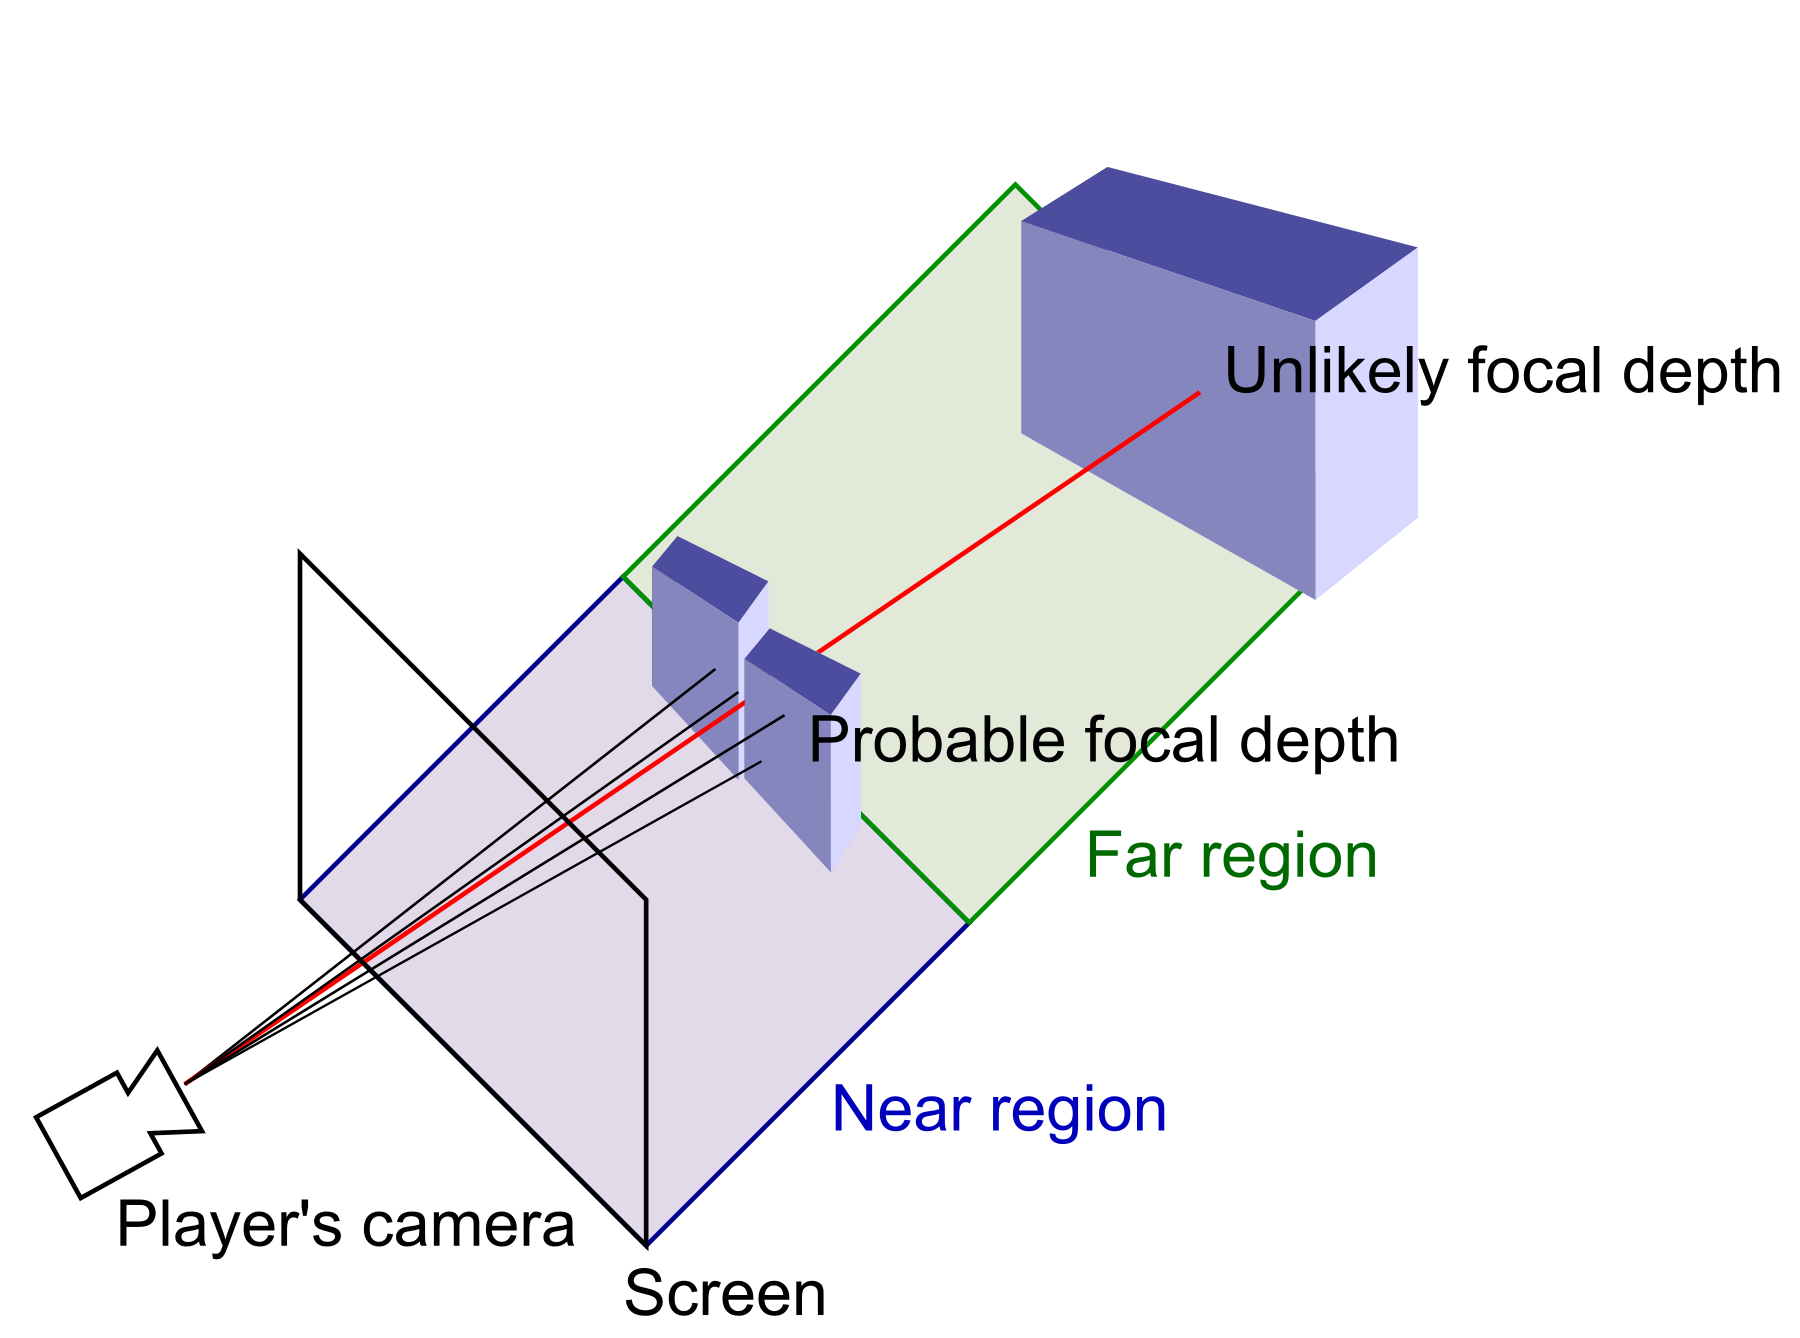
\includegraphics[width=0.45\textwidth]{images/distanceCheck.png}
            \caption{In order to avoid focusing at unlikely depths (red), multiple rays (black) are cast to find $d_f$ .}
            \label{fig:raycast}
\end{figure}

For each pixel, we find the depth $d_p$ of the object under that pixel. In order to avoid \say{bleeding effects} we split the screen into two regions: near and far, before convolving the set of pixels in each of these regions against a circular blur kernel with a fluctuating radius $r \propto | d_f - d_p |$. The opacity of the kernel is inversely proportional to $r$. These regions are then merged to create the completed frame. We do not immediately change $d_f$ when participants move or look around. Instead, we interpolate the change in focal distance based on the refocusing speed of the human eye~\cite{sun88} to more accurately mimic behaviours of the human visual system. We selected the radius $r$ using a preliminary experiment where a test environment was generated consisting of multiple identical objects at differing visual depths, as shown in Fig.~\ref{fig:testScene}. Through visual analysis of this scene, $r$ was selected to be 1.75\% of the screen width. We assume a fixed inter-pupillary distance (IPD) equal to the average value for adults.  \\
%
%\begin{figure}[h!]
%        \centering
%            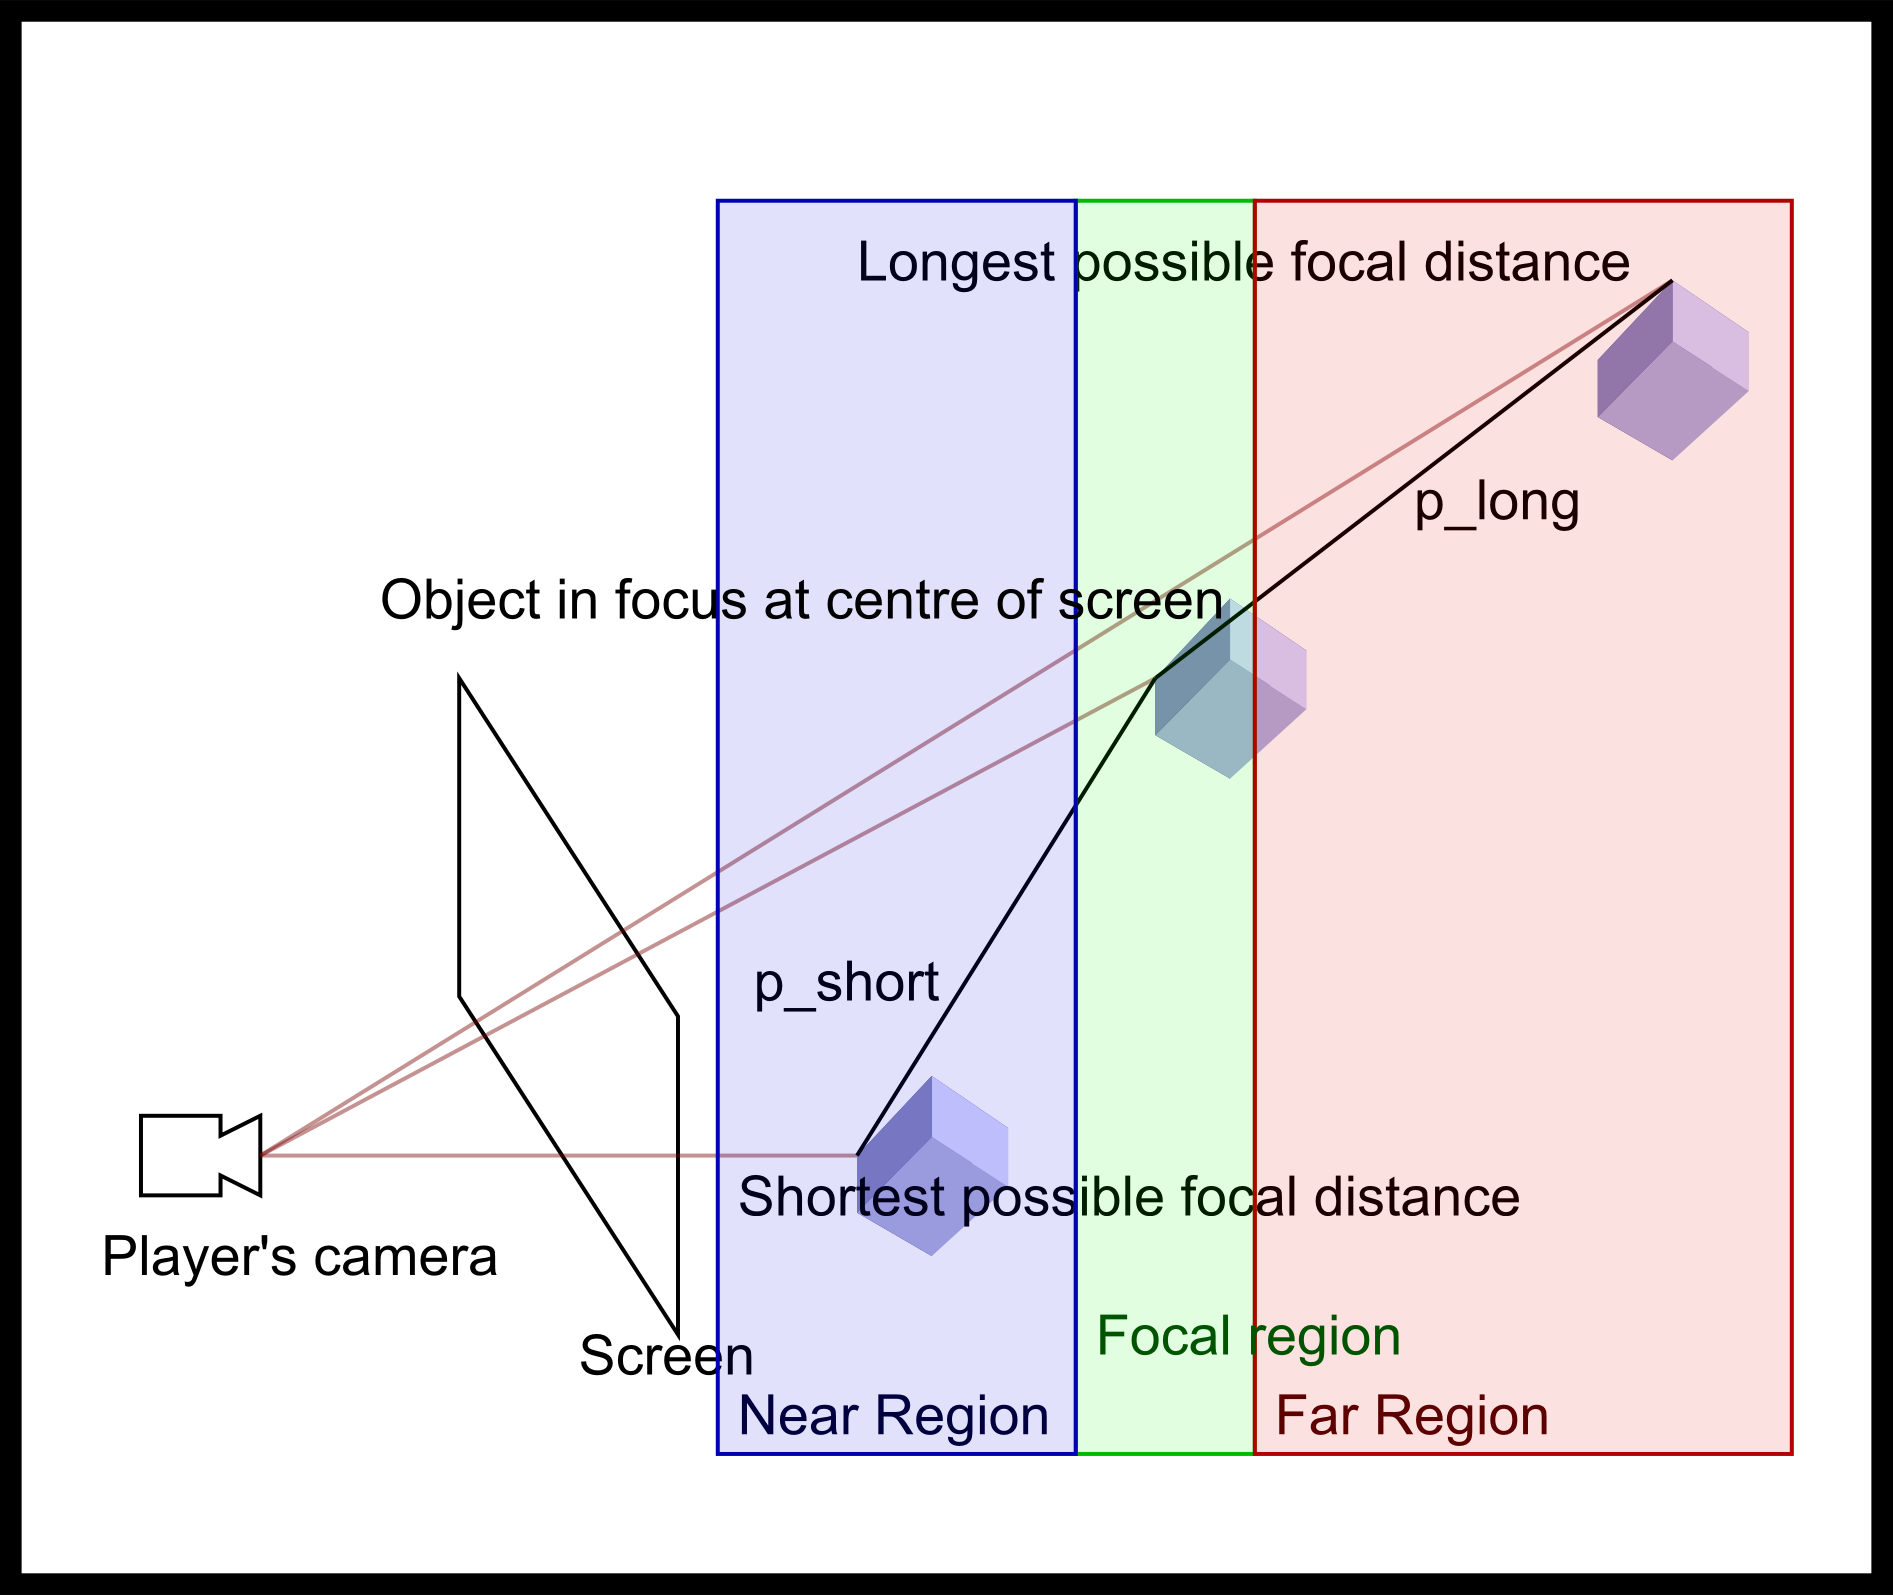
\includegraphics[width=0.45\textwidth]{images/bokehDOF.png}
%           \caption{The setup for bokeh DoF. {\color{blue} [TODO: caption]}}
%            \label{fig:raycast}
%\end{figure}
%
%We then split the screen into three regions: the near, far and focal regions. The focal region is the set of pixels whose object distances are within $100cm$ of $d_{centre}$. The far region consists of all pixels with object distances further than this, and the near; all pixels with smaller object distances.\\

%For each pixel in the near region, we define $p_c$ as the world space distance between the object under the pixel and the object under the pixel at the centre of the screen. We then construct a Circle of Confusion for each pixel, using a textured quad containing a circular bokeh opacity texture. This circular texture has a radius $r = D_c * \frac{p_c}{p_{short}}$ and an opacity proportional to this radius. \\
%
%To move the focal regions we cast a ray from the center of the participants stereo 3D view on the Oculus into the scene, and find the distance $D$ at which this ray first intersects an object. We then create a circle of radius $r_c = \frac{D}{C_c}$ ($C_c$ is constant) and randomly cast $n$ rays into this circle, with a weighting towards rays clustered in the center, each of which reports a distance $d_{0..n}$. We then iteratively cull outlier distances from this set and take the mean distance until a confident final focal distance $d_f$ is found. $d_f$ is then compared to the prior focal distance and interpolated based on .\\
%
%\begin{figure}[h!]
 %       \centering
 %           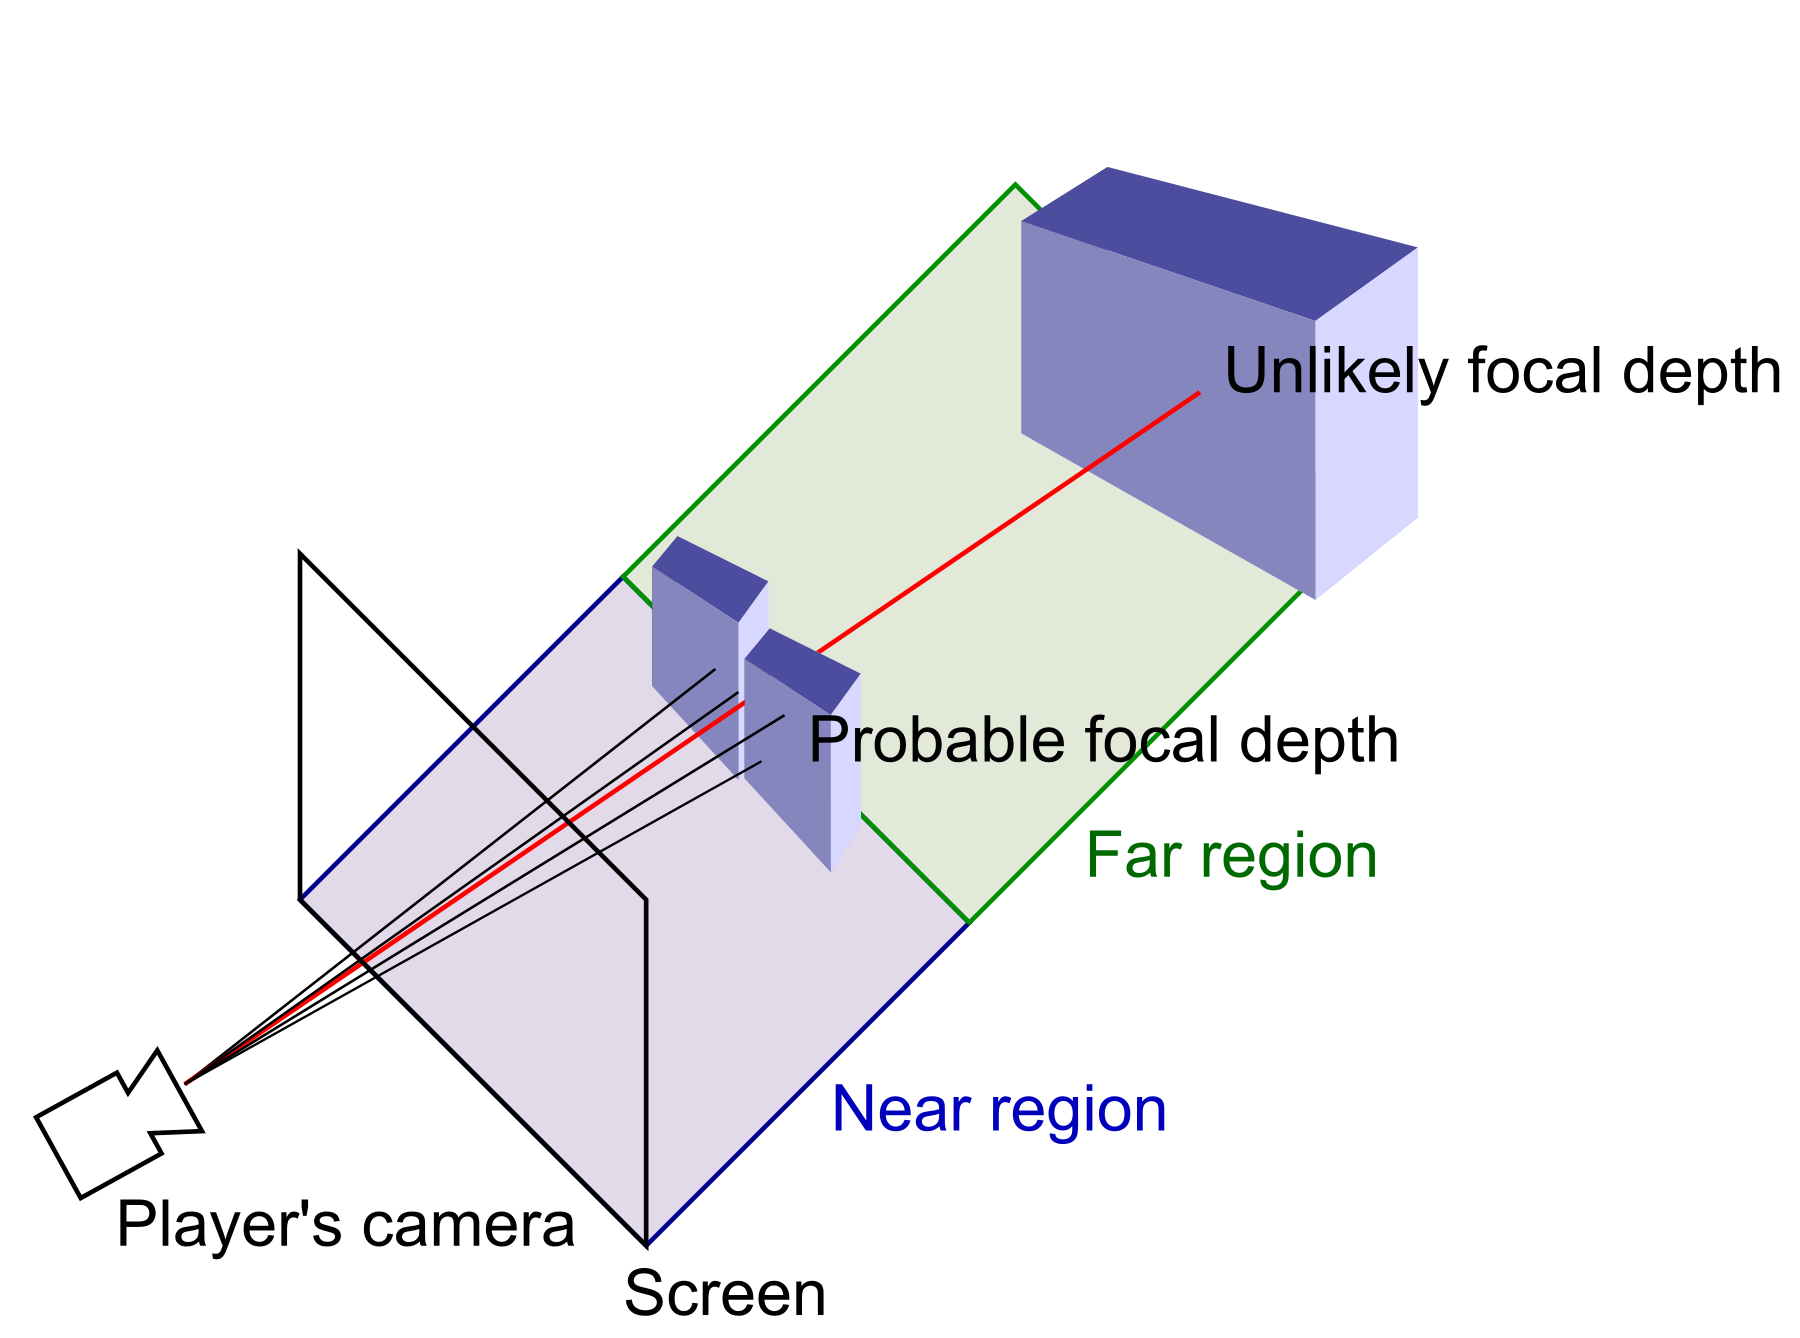
\includegraphics[width=0.45\textwidth]{images/distanceCheck.png}
%            \caption{In order to ensure focus on the correct object, rays (grey) are cast into the circle around the object under the centre of the screen (black ray).}
%            \label{fig:bokeh}
%\end{figure}
%REWORDING END


Participants completed the study on a machine running Windows 7 with 8GB RAM, a 3.6GHz Intel quadcore CPU and a NVIDIA GTX 770 GPU with an attached Oculus Rift DK1 HMD. An example picture of the experimental set-up is shown in Fig.~\ref{fig:user}. 
\\

\begin{figure}[h!]
        \centering
            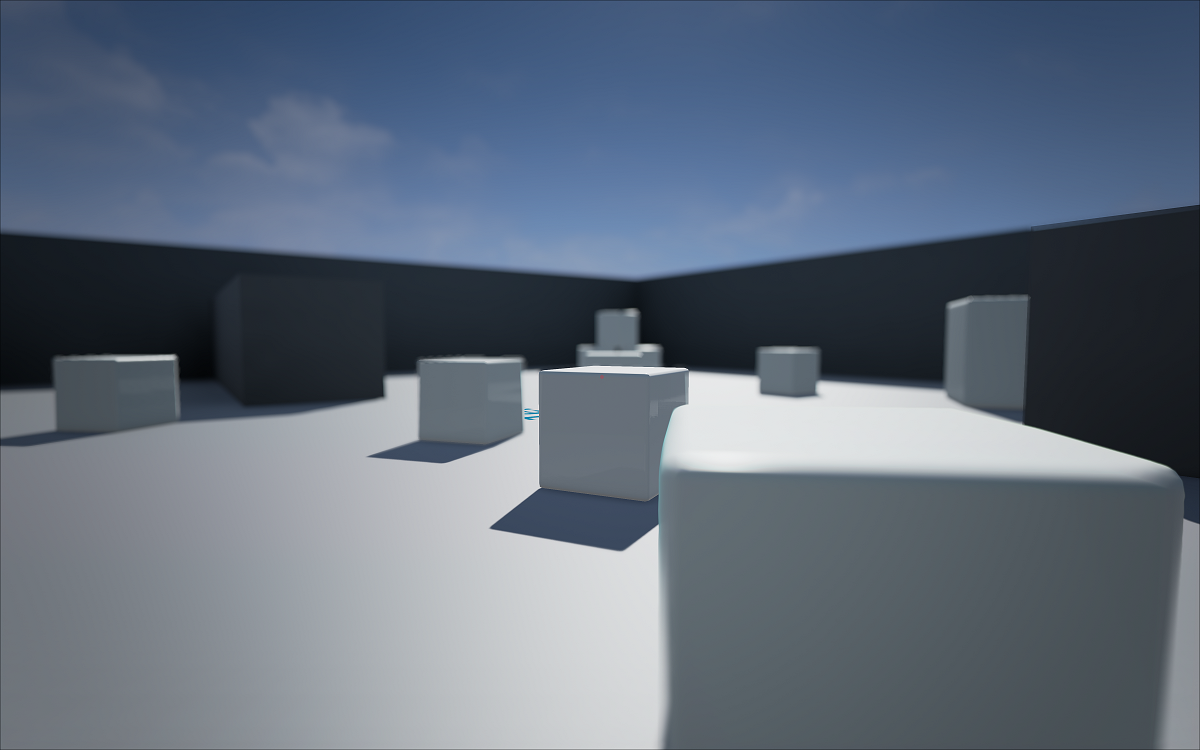
\includegraphics[width=0.45\textwidth]{images/testScene.png}
            \caption{The test scene used for selecting DoF blur radius}
            \label{fig:testScene}
\end{figure}

% thrhee comment: the following needs to be removed
% We utilize the bokeh DOF provided in provided in UE4 as the UE4 implementation is both high quality and fast. The above process is completed at quarter resolution (half vertical and horizontal). No artefacts or errors are visible from this, due to the low resolution of the Oculus screen.\\

% no fine detail
% focal gradient / etc


% The followings are not required
% We chose the Oculus DK1 over more recent devices, such as the Oculus DK2 due to the lower hardware requirements to optimally run the DK1. Furthermore, the DK2, being newer, does not have the same level of software support that the DK1 offers, and was at the time of our study, known to have performance issues.{\color{blue}[Do I need to cite this?]}. An example picture of the experimental set-up is shown in Figure \ref{fig:user}\\

\begin{figure}[h]
        \centering
            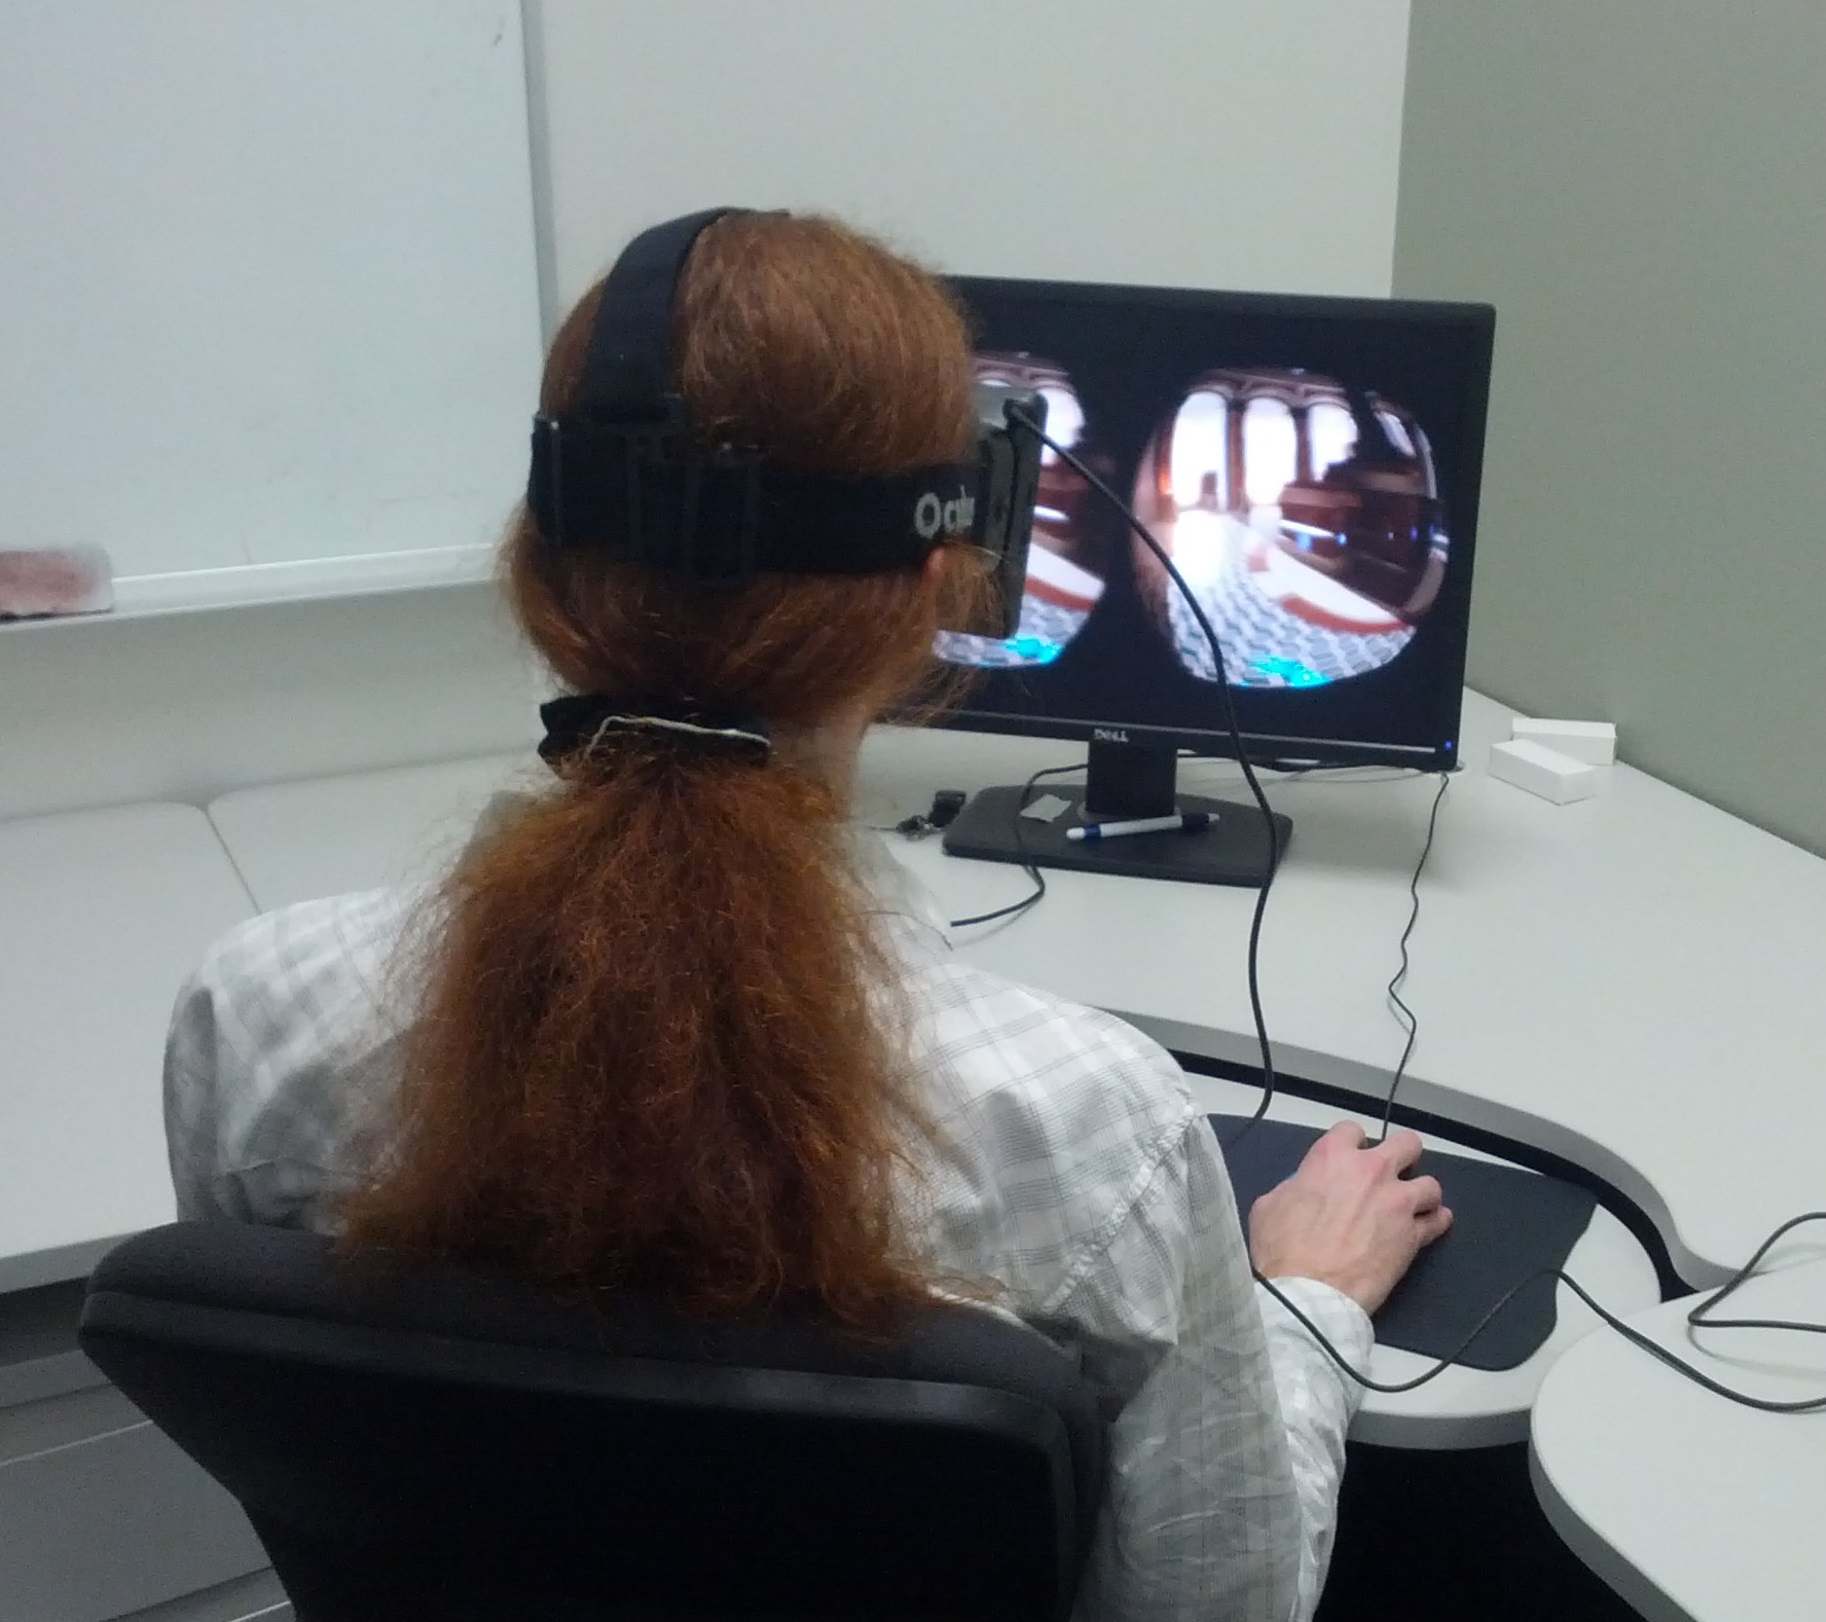
\includegraphics[width=0.45\textwidth]{images/participantv2.jpg}
            \caption{A participant during the user study.}
            \label{fig:user}
\end{figure}


\section{Stimuli}

% The referenced figure was moved to the related work section to make it render on page 3 properly

Participants in our study were shown two scenes: a temple and a mountainous landscape. Example screenshots are shown in Fig.~\ref{fig:temple1}. These specific scenes were chosen in order to represent broad VR applications. The temple scene consists of primarily near focal distances, with three separate rooms with different illuminations: bright, natural and dark. All three rooms had high detail objects that a user could pay close attention to at close range. The mountainous landscape in contrast, consists of primarily far focal distances with few high detail objects. 
%Both are modified from freely available Unreal Engine demos. 
\\

A total of 16 participants took part, with an age range of 18 to 25 years old. Three participants were female and the rest were male. Participants interacted with the two scenes using a control scheme proposed by Valve software~\cite{valveVR}: the view vector of the Oculus is independent to the motion vector of the user's virtual avatar. The user controls the movement of their avatar using the keyboard to move forwards or backwards, or strafe left and right, and they use the mouse to rotate their avatar's torso.  Based on recommendations from~\cite{oculus}, jumping is disabled, and the user is limited to a velocity of $1.4ms^{-1}$, to minimise discomfort arising from factors related to traversing the virtual environment. Similarly, if a user's velocity has a non-zero vertical component (such as when they walk up stairs), their horizontal velocity is decreased to compensate, keeping their total velocity constant.\\
% Mention that this is done to reduce the discomfort impact of vertical motion

Participants were given minimal direction in what they were to do in the virtual scene: they were simply instructed to explore. This was done instead of specifying a track to follow as we wanted participants to move around these environments naturally. Participants were allowed to withdraw from the experiment at any time if they felt too sick.\\

\section{Procedure}

\begin{figure*}[th]   
    \noindent
        \centering
            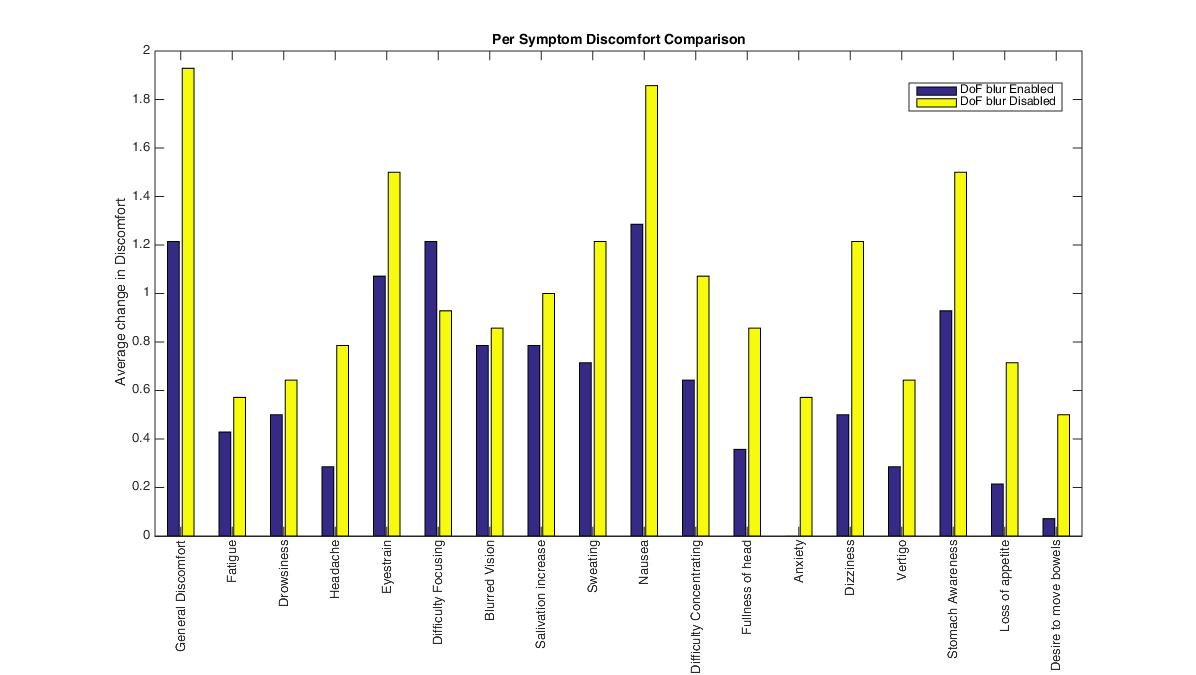
\includegraphics[width=\textwidth]{images/perSymptom.jpg}
            \caption{A comparison between average of participant responses with DoF blur enabled and disabled.}
            \label{fig:sicknessBreakdown}
\end{figure*}


Participants involved in the study were invited to two sessions on sequential working days. In the first session, the participant was shown the two scenes in a random order, with DoF blur applied to one randomly chosen scene. In the second session, the DoF blur was applied to the other scene, and the ordering of the scenes was reversed. The number of participants whose first session had DoF blur enabled was equal to the number of participants whose first session had DoF blur disabled.\\
% minor rearrange needed to fit

For this study, we used a SSQ consisting of 18 questions. For each question, the participant is verbally asked as to their current experience of a symptom, using a 5 point Likert scale (ranging from \say{None}, indicating no presence of that particular symptom, to \say{Severe}, indicating severe or traumatic presence). The SSQ responses resulted in a 18 part measurement of subjective discomfort across specific symptoms, as well as a \textbf{\textit{total sickness measure}} derived from the sum of user responses, multiplied by weights used by~\cite{kennedy93}.\\

At the beginning of each session, participants were asked to complete a SSQ. They then put on the Oculus and adjusted its physical settings to be comfortable. Participants with glasses were given the option to wear them inside the Oculus if they could fit, otherwise the appropriate lenses were put into the Oculus to compensate.\\

The nature of the control scheme was then explained to each participant. They were given a minute to get used to how the controls worked, and then explored whichever scene had been randomly chosen for 15 minutes. A SSQ was then verbally completed. Participants were asked to close their eyes, and were relocated to the other scene, which they then explored for another 15 minutes before completing the third SSQ and taking off the Oculus. They were then asked to relax and wait 15 minutes, before completing a final SSQ. Each SSQ was administered verbally.\\



\section{Results}

\subsection{Observation}

In each session we recorded four SSQ results: the initial response, post scene one, post scene two, and 15 minutes after final exposure to the second scene on the Oculus. We subtract the initial response from each of the three later responses to give a difference score for the severity of each symptom.  The individual symptoms are multiplied by weights and summed to give the total sickness measure $S_T$~\cite{kennedy93} that the participant experienced during the session. The changes in total sickness measure $\Delta S_T$ is then used as a metric for determining visual discomfort on the HMD: a higher $\Delta S_T$ indicates the user experienced a greater increase in discomfort during their session. \\

Our study found a statistically significant reduction on total sickness measure when dynamic DoF blur was enabled, compared to when it was not, after analysis using one-way within-subjects Analysis of Variance (ANOVA) on reported $\Delta S_T$: $ (F(1,18) = 7.64$, $p < 0.0133)$. 
%
The presence of DoF blur, as shown in Fig.~\ref{fig:sicknessBreakdown} and ~\ref{fig:totalSicknessScore} was found to be effective in reducing visual discomfort in users of HMDs. A reduction of mean total sickness measure was observed, decreasing from 16.83 to 11.82 when DoF blur was enabled, with a consistent standard deviation of approximately 13.
%
Five participants ended up withdrawing from one of their sessions, and one participant's results had to be discounted due to a recording error. \\

\subsection{Analysis}

Based on previous studies, an effective system for reducing the contribution of the accommodation-vergence conflict on visual discomfort should: reduce the area of the screen that is in focus at any given time, thereby reducing amount of focusing a user needs to do; reduce the range of virtual depths a user must focus on; or minimize the rate at which the user must adjust their vergence. Our system was constructed to meet the first two of these conditions.\\

A decrease in mean sickness measure for each of the three discomfort categories~\cite{kennedy93} was observed. Mean nausea discomfort decreased from 8.43 to 5.48, mean oculomotor discomfort decreased from 5.79 to 4.27 and mean disorientation discomfort decreased from 7.65 to 5.07 when DoF blur was enabled, compared to when it was disabled. Figure~\ref{fig:categorySickness} shows the aggregate results for participants responses, split into these three categories. The consistent decreases in discomfort symptom severity show that our system is effective at alleviating the accommodation-vergence conflict and its impact on visual  discomfort.\\

The average discomfort participants reported throughout their sessions was consistently lower when DoF blur was enabled: all symptoms decreased except for \say{difficulty focusing}, as shown in Figure~\ref{fig:sicknessBreakdown}. The nature of this symptom is complicated, as differing interpretations may lead to different responses. If a participant is easily able to focus on a screen that displays blurry content, we expect them to state they have no difficulty focusing. Participants may however, interpret the blurry screen content as being difficult to focus on, as they associate viewing blurry visual stimuli with focusing difficulties, especially on immersive HMDs where they do not have external stimuli to provide visual reference. A clarification to the SSQ used is required to eliminate this uncertainty.\\ 

\begin{figure}
        \centering
            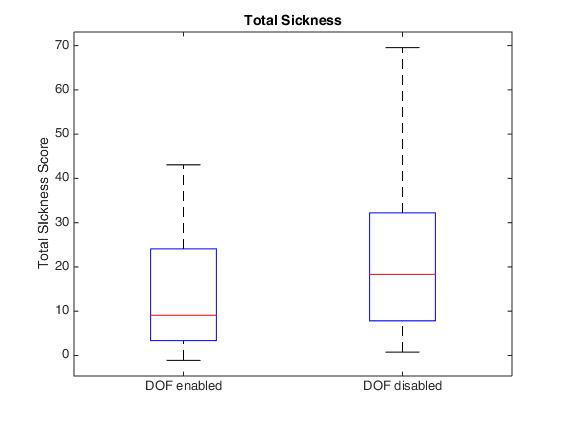
\includegraphics[width=0.5\textwidth]{images/total.jpg}
            \caption{Total sickness score for participants with (left) and without (right) DoF enabled.}
            \label{fig:totalSicknessScore}
\end{figure}


\begin{figure*}[t]
        \centering
            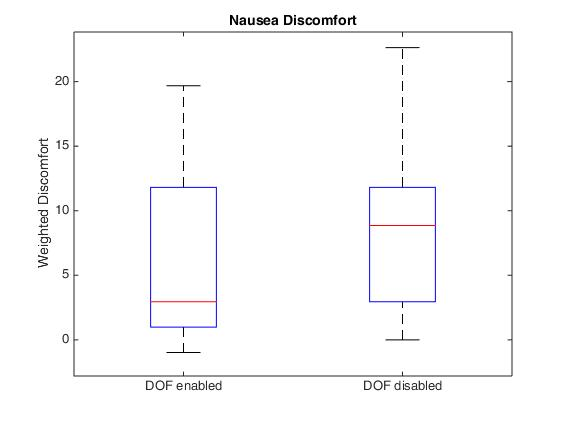
\includegraphics[width=0.32\textwidth]{images/nausea.jpg}
            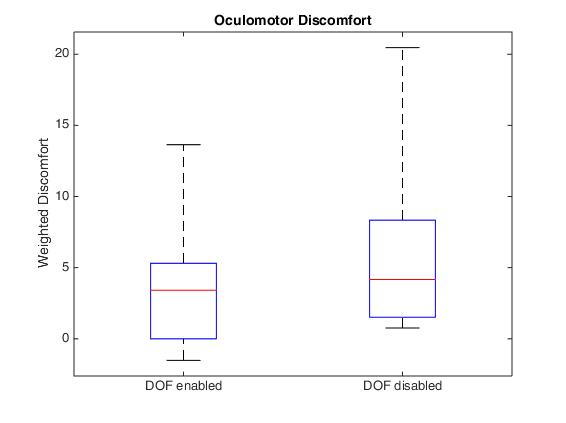
\includegraphics[width=0.32\textwidth]{images/oculomotor.jpg}
            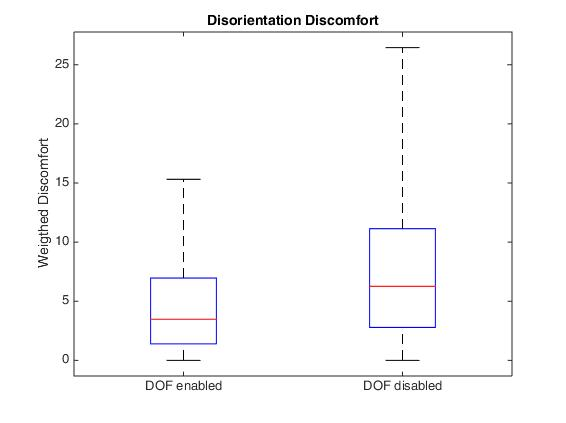
\includegraphics[width=0.32\textwidth]{images/disorientation.jpg}
            \caption{Change of sickness measure for each of the three discomfort categories: Nausea (left), Oculomotor (centre), Disorientation (right).}
            \label{fig:categorySickness}
\end{figure*}


Not all of the questions asked during our experiment were used to calculate sickness measures: anxiety and drowsiness responses were instead used to give a quantifiable estimation of a participant's mental state during the experiment. The loss of appetite and desire to move bowels results were also not used, as it was not feasible to control external factors such as time since the participant had last eaten, which were considered to significantly contribute to participant responses to these symptoms. \\

All of the participants who withdrew during our experiment did so in their first session, and every one of these sessions was one in which DoF blur was not enabled. Three of the withdrawals in the experiment occurred on unusually warm days; interior temperature was significantly higher than normal. The lab where this experiment was situated does not have an effective climate control system.\\

% moved to disucssion 
% There were a total of two participants who stated \say{(they) felt equally sick on both sessions}, and had consistent responses to their discomfort symptoms on each session. This indicates that there are people for whom DoF blur is not always relevant for reducing visual discomfort on HMDs: reducing the contribution of the accommodation-vergence conflict does not significantly affect overall their visual discomfort. 

% Possible reasons for this may include: these individuals were not well suited to the chosen HMD parameters (for example, they may have a IPD that differs significantly from the average), or they experienced an adverse reaction to a HMD factor that we did not explore which overpowered the contribution of the accommodation - vergence conflict to discomfort.

\section{Conclusions and Discussion}

% \textbf{Summary} do not need to specify
This paper presents a psychophysical experiment used for evaluating the effectiveness of DoF blur on visual discomfort on immersive HMDs like the Oculus. We find that DoF blur decreases overall visual discomfort on HMDs, when tested on dynamic, interactive scenes.\\

% \textbf{Analysis of effectiveness of DOF blur in HMD}: do not need to specify
We implemented dynamically adjusted DoF of the rendered scene on the Oculus such that the centre of the virtual view-port formed by combining the stereo 3D screens always remains in focus to the user. Our DoF implementation discourages the users focusing in regions outside the centre of the screen as well as discouraging focusing on objects that are at significantly different depths to the current focal distance, as they are blurred. This mitigates the accommodation-vergence conflict in the human visual system and mimics peripheral blur that is absent on typical LCD viewing.\\

In general stereo displays (e.g. LCD), limiting eye movement to only focusing on the centre of a screen will limit users' spatial degrees of freedom. However, in HMDs, the majority of spatial movement will occur through head movements (i.e., changing the orientation of the Oculus to look somewhere else) rather than through eye movements, compensating for this drawback.\\

There were a total of two participants who stated \say{(they) felt equally sick on both sessions}, and had consistent responses to their discomfort symptoms on each session. This indicates that there are people for whom DoF blur is not always relevant for reducing visual discomfort on HMDs: reducing the contribution of the accommodation-vergence conflict does not significantly affect overall their visual discomfort. \\


We used a common HMD, with display settings optimised for an average human, with a mouse and keyboard control scheme implemented in many VR applications. As this control scheme is not ubiquitous and the average settings will not work optimally for all users, further experiments should allow more user fine-tuning of the display and control settings.\\

% It is not required to mentioned
% Further experiments for determining discomfort should be conducted on climate controlled rooms to eliminate potential external variables. \\


%\section{Ramblings and notes}
Stuff in here won't render, but is included so i can easily add them in as required.

\cite{Toyoura:2012:MPD:2407516.2407526} created a HMD in which the DOF was controllable by the user to convey depth. Using a spatial dextirity task as a metric, they show inconsistant improvements in task completion time for some participants but report no overall improvement.\\


the first occurrence of Simulator Sickness was reported on the first helicopter fight simulator, back in 1956 \cite{miller}\\

	Simulator sickness is referred to as the incidence of sickness symptoms associated with motion sickness, arising in the specific case where the user is interfacing with a visual display\cite{johnson}. \\


	

	It has been proposed that the disassociation of the vergence and accommodation depth cues in the human visual system when stereoscopic displays are utilized is a significant factor contributing to simulator sickness \cite{howard:depthPerception}. \\  

	
Viirre and Bush (2002) pointed out indirect effects of VE on the 
visual system (i.e., eyestrain, changes in binocular vision, and 
visual acuity), balance, motion detection, nausea, and motion 
sickness.


	
	
 Banks, Akeley, Hoffman, and Girshick (2008) found performance at an orientation detection task improved when blur was appropriate for the convergence 

\bibliographystyle{ieeetr}
\bibliography{references}
%\printbibliography

\end{document}
